%
% Szablon, v. 2.0
% p.wlaz@pollub.pl
%



\documentclass[12pt]{mwbk}


%%%%%%% marinesy, rozmiary, to warto dopasować do drukarki
\usepackage[a4paper,twoside,top=2.6cm,bottom=2.6cm,inner=3cm,outer=2.6cm]{geometry}

%%%%%%%% polszczyzna
\usepackage[OT4]{polski}


%%%%%%%%% sposób kodowania literek w edytorze
\usepackage[utf8]{inputenc}

\usepackage[font=small,labelfont=bf,justification=centering]{caption}


%%%% gdyby ktoś chciał powyklejać z~pedeefa
%%%% teksty za pomocą AcroReadera, to cmap.sty
%%%% pomoże w~prawidłowym działaniu z~polskimi literkami
%%%% Może to być przydatne, gdyby ktoś na podstawie
%%%% elektronicznej wersji chciał przygotować dane do 
%%%% badania antyplagiatowego
%% \usepackage{cmap}

%%%%%%%%%%%%%%%%%%%%%%%%%%%%%%%%%%%%%
%%%%% jeśli chcesz by główny tekst oraz wzory matematyczne były
%%%%% składane czcionką typu Times Roman (w~odróżnieniu od standardowej
%%%%% TeXowej, czyli Computer Modern Roman) to linia poniżej
%%%%% ma być 'aktywna', jeśłi postawisz na jej początku znak %
%%%%% to uzyskasz skład tą tradycyjną czcionką typu 
%%%%% Computer Modern Roman mającą wielu wiernych
%%%%% fanów w~świecie TeXa). Konsekwencją jednak będą zmiany
%%%%% rozmiarów czcionek dla rozdziałó i podrozdziałów - rzecz bez większego
%%%%% znaczenia, wynikająca z pewnych zaszłości historycznych (ComputerModern
%%%%% niegdyś były używane wyłącznie w postaci tzw. bitmap)
%% \usepackage{mathptmx} \usepackage{tgtermes}




%%%%%%%%%%%%%% pozostałe pakiety używane w~pracy, to już zależy od
%%%%%%%%%%%%%% autora, więc może być tego więcej
\usepackage{fancyhdr}
\usepackage{graphicx}
\usepackage{amsmath}
\usepackage{amsthm}
\usepackage{amssymb}
\usepackage{url}
\usepackage{longtable}
\usepackage{array,hhline}

%%%%%%%% hyperref po to by przeglądarka pedeef ukazywala na odwołania
%%%%%%%% prawidłowo skonstruowane za pomocą \ref, \cite i.t.d. jako
%%%%%%%% hiperłącza
%% \usepackage{hyperref}



%%%%% dla fanów ``profesjonalnych'' tabel w~stylu zachodnich książek

\usepackage{booktabs} \heavyrulewidth=1.5bp \lightrulewidth=0.5bp


%%%%%%%%%%% poniżej uniwersalny sposób na ucywilizowanie znaków 
%%%%%%%%%%% niewiększości, niezależny od pakietu {polski}, ale za to 
%%%%%%%%%%% zależny od {amssymb}, ma tą zaletę, że działa np. z Timesem
%%%%%%%%%%% w matematyce
\let\leq\leqslant\let\le\leq\let\geq\geqslant\let\ge\geq


%%%%%%% jeżeli będziesz chciał włączać do swojej pracy fragmenty programów, 
%% to kilka ponizszych linijek przyda się, jeśli nie - usuń je
\usepackage{listingsutf8}
\usepackage{color}
\definecolor{siwy}{gray}{0.95}
\lstset{extendedchars=true, inputencoding=utf8/latin2, language=octave,
	basicstyle=\footnotesize, frame=single,
	backgroundcolor=\color{siwy},
	numbers=left, numberstyle=\tiny\bf, numbersep=5pt, stepnumber=1}


%%%%%%%%%%%%%%%%% struktury do tworzenia twierdzeń i~tym podobnych

\theoremstyle{plain}
\newtheorem{twier}{Twierdzenie}[chapter] % pierwsze to nazwa środowiska,
                                      %drugie to wyświetlana nazwa
				% to trzecie w~nawiasie kwadratowym
				% wskazuje numer dolepiony z~lewej do
				% numeru twierdzenia (tu numer
				% 'chapter', 
\newtheorem{lemat}{Lemat}[chapter]

\theoremstyle{definition}
\newtheorem{defi}{Definicja}[chapter]

\theoremstyle{remark}
\newtheorem{uwaga}{Uwaga}[chapter]
\newtheorem{wniosek}{Wniosek}[chapter]

%%%%% więcej możliwości w~dokumentacji amsthm



%%%%%%%%%%%%%%%%%%%%%%%%%%%%%%%%%%%%%%%%%5
%%%%%%%%%%%%%%%%%%%%%%%%%%%%%%%%%%%%%%%%%%
%%%%%%%%% wcięcie akapitowe %%%%%%%%%%%%%%
%%%%%%%%%%%%%%%%%%%%%%%%%%%%%%%%%%%%%%%%%%
%%%%%% ustawić w~zaleceń i~gustu %%%%%%%%%
%%%%%%%%%%%%%%%%%%%%%%%%%%%%%%%%%%%%%%%%%%
%%%%%%%% zalecenie na stronie wydziałowej
%%%%%%%% było 1.25cm i wyglądało jakoś 
%%%%%%%% śmiesznie duże, więc spłoszony nieco
%%%%%%%% wpisałem 1cm, ale uważny czytelnik już
%%%%%%%% zapewne się domyśli, że podmiana napisu 
%%%%%%%% =1cm na =1.25cm sprawi, że wcięcia na początku
%%%%%%%% akapitu ustawią się na (nieco przydużą)
%%%%%%%% wartość 1.25cm 

\parindent=1cm



%%%%%%%%%%%%%%%%%%%%%%%%%%%%%%%%
%%%%% tu pewne poluzowanie rozmieszczenia elementów tabelek
%%%%% możecie sobie poeksperymentować, by dopasować do swych
%%%%% gustów, a przede wszystkim gustów promotorów (promotorek)
  \tabcolsep=4mm          
  %\renewcommand\arraystretch{1.3}
%%%%%%%%%%%%%%%%%%%%%%%%%%%%%%%%%%



%%%%%%%%% teraz żywa pagina (aka 'running headline') i~numerowanie stron
%%%%%%%%%%%%%%%%%%%%%%%%%%%%%%%%%%%%%%%%%%%%%%%%%%%%%%%%%%%%%%%%%%%%%%%%
%%%%%na górze mają być śródtytuły, na dole (po stronie zewneętrznej)
%%%%%numery stron. Poszedłem kapkę dalej i~na stronach ropoczynających
%%%%%rozdział nie ma paginy (górki).
%%%%% Oczywiście jeśli ostatnia strona
%%%%% jest pusta (uzupełnia jeno parzystość) to tam żadnej stopki ani 
%%%%% górki byc mnie może - ma być pusta.
%%%%%%%%%%%%%%%%%%%%%%%%%%%%
\pagestyle{fancy}
\fancyhead{}% oczyszczenie
\fancyhead[RO]{\rightmark} %% na nieparzystych 'podległe' śródtytuły
\fancyhead[LE]{\leftmark} %% na parzystych 'ważniejsze'
\fancyfoot{}% oczyszczenie
\fancyfoot[RO,LE]{\arabic{page}}  %% numer na dole (po prawej na
%% nieparzystych, po lewej na parzystych)
\renewcommand\headrulewidth{0.4pt} %%% cienka hrulka oddzielająca paginę
                                    %%% od kolumny tekstu
\fancypagestyle{closing}{%%%%%% to styl dla stron zamykających rozdział
\fancyhead{}% oczyszczenie
\fancyhead[RO]{\rightmark} %% na nieparzystych 'podległe'
\fancyhead[LE]{\leftmark} %% na parzystych 'ważniejsze'
\fancyfoot{}% oczyszczenie
\fancyfoot[RO,LE]{\arabic{page}}  %% numer na dole (po prawej na
                                  %% powyższą linijkę usuń jeśli nie
				  %% chcesz numerów na niepełnych
				  %% kolumnach (zamykających rozdział)
\renewcommand\headrulewidth{0.4pt}
}
\fancypagestyle{opening}{%%% styl stron rozpoczynających rozdział
\fancyhead{}% oczyszczenie
\fancyfoot{}% oczyszczenie
\fancyfoot[RO,LE]{\arabic{page}}  %% numer na dole (po prawej na
\renewcommand\headrulewidth{0pt}
}
\fancypagestyle{plain}{%%%% styl zwykły, niektóre konstrukcje
                       %%%% (typu \titlepage, którego ja tu nie używam
                       %%%% ale może są jakieś inne o których nawet nie chce 
                       %%% mi się myśleć, więc dla spokoju robię to po swojemu
\fancyhead{}% oczyszczenie
\fancyfoot{}% oczyszczenie
\fancyfoot[RO,LE]{\arabic{page}}  %% numer na dole (po prawej na
\renewcommand\headrulewidth{0pt}
}

%%%%%%%%%%%%%%%%%%%%%%%%%%%%%%%%%5
%%%%%%%%%%%%%%%%%%%%%%%%%%%%%%%%%%
%%% lekka modyfikcja 'markow' do paginy
%%% uznalem, ze jesli ktos nie da \section (np we wstepnie czy
%%% podsumowaniu to niech na obu sronach w~paginie pojawia sie tytuł
%%% chaptera, bo standardowo, to na nieparzystej stronie w takiej sytuacji
%%% nad górną linią ziałaby pustka, co mogłoby wprowadzać konsternację
\makeatletter
    \def\chaptermark#1{%
      \markboth{%
        \ifHeadingNumbered
     \if@mainmatter
     \@chapapp\
            \thechapter.\enspace
          \fi
        \fi
        #1}{%
        \ifHeadingNumbered
     \if@mainmatter
     \@chapapp\
            \thechapter.\enspace
          \fi
        \fi
        #1%
	}}%
    \def\sectionmark#1{%
      \markright{%
        \ifHeadingNumbered \thesection.\enspace \fi
        #1}}
%%%%%%%%%%%%%%%%%%%%%%%%%%%%%%%%%%%%%%%%%%%%%%%
%%%%%%%%%%%%%%%%%%%%%%%%%%%%%%%%%%%%%%%%%%%%%%%%
%%%%%%%%%%%% wielkości czcionek dla chapter i~section
%%%%%%%%%%%% 16 dla rozdziału, 14 dla podrozdziału - te domyślne
%%%%%%%%%%%% w klasie mwbk były całkiem ładne, ale żeby nie było
%%%%%%%%%%%% że nie potrafię ustawić
%%%%%%%%%%%%%%%%%%%%%%%%%%%%%%%%%%%%%%%%%%%%%%%%%%%
\SetSectionFormatting[breakbefore,wholewidth]{chapter}
        {0\p@}
        {\FormatRigidChapterHeading{6.4\baselineskip}{12\p@}%
	{\large\@chapapp\space}{\fontsize{16}{19}\selectfont}}
        {1.6\baselineskip}
\SetSectionFormatting{section}
        {24\p@\@plus5\p@\@minus2\p@}
	{\FormatHangHeading{\fontsize{14}{16}\selectfont}}
        {10\p@\@plus3\p@}
\makeatother	



%%%%%%%%%%%%%%%%%%%%%%%%%%%%%%%%%%%%%%%%%%%%%%
%%%%%%%%%%%%%%%%%%%%%%%%%%%%%%%%%%%%%%%%%%%%%%
%%%%%%%%%%%%%% jakies inne pomocnicze definicje, ja na przykład lubię
% \R
%%%%%%%%%%%%%%%%%%%%%%%5
%%%%%%%%%%%%%%%%%%%%%%%
%%%% tak naprawdę są t potrzebne tylko po to
%%%% by zadziałały przykłady poniżej w tekście
%%%% które w sposób dość losowy zostały 
%%%% pobrane z jakichś moich starych plików
%%%%%%%%%%%%%%%%%%%%%%%%%%%%%%%%%%
%%%%%%%%%%%%%%%%%%%%%%%%%%%%%%%%%%%
%%%% w realnej pracy te poniższe śmieci możecie oczywiście
%%%% usunąć
%%%%%%%%%%%%%%%%%%%%%%%%%%%%
\newcommand\R{\mathbb{R}}
\newcommand{\ff}{\mathbf{f}}
\newcommand{\hh}{\mathbf{h}}
\newcommand{\xx}{\mathbf{x}}
\newcommand{\yy}{\mathbf{y}}
\newcommand{\zz}{\mathbf{z}}
\newcommand{\gggg}{\mathbf{g}}
\newcommand{\skalar}[2]{\pmb{\langle}#1,#2\pmb{\rangle}}
%%%%%%%%%%%% koniec tych dodatkowych definicji

%%%%%% trocę więcej ``luzu'' przy rozmieszczaniu {fgur} i~{table}

 \renewcommand{\topfraction}{0.9}	% max fraction of floats at top
    \renewcommand{\bottomfraction}{0.8}	% max fraction of floats at bottom
    %   Parameters for TEXT pages (not float pages):
    \setcounter{topnumber}{2}
    \setcounter{bottomnumber}{2}
    \setcounter{totalnumber}{4}     % 2 may work better
    \setcounter{dbltopnumber}{2}    % for 2-column pages
    \renewcommand{\dbltopfraction}{0.9}	% fit big float above 2-col. text
    \renewcommand{\textfraction}{0.07}	% allow minimal text w. figs
    %   Parameters for FLOAT pages (not text pages):
    \renewcommand{\floatpagefraction}{0.7}	% require fuller float pages
    % N.B.: floatpagefraction MUST be less than topfraction !!
    \renewcommand{\dblfloatpagefraction}{0.7}	% require fuller float pages
    % remember to use [htp] or [htpb] for placement

    
%%% DWA proste polecenia służące do ujednolicenia podawania źródeł przy rysunkach i~tabelkach    
    
    \newcommand\zrodlo[1]{\par\vspace{-3mm}{\small\textit{Źródło: }#1 }}
    \newcommand\zrodlotab[1]{{\par\vspace{2mm}\small\textit{Źródło: }#1 }}

\raggedbottom   %%% to znaczy, że nie będzie siłowego wyrównywania typowych
                %%     stron do jednakowej wysokości

\linespread{1.3}
\begin{document}

%%%%%%%%%%%%%%%%%%%%%%%%%%%%%%%%%%%%%%%%%
%%%%%%%%%%%%%%%%%%%%%%%%%%%%%%%%%%%%%%%%%
%%%%%%%% STRONA TYTUŁOWA %%%%%%%%%%%%%%%%

\thispagestyle{empty}  % tu wszak nie chcemy żadnej numeracji stron


%%%%%%%%%%%%%%%%%%%%%%%%%%%%%%%%%%%%%%%%%%%%%%%%%%%%%%%%%%%%%%%
%%%%%tytuły definiuje jako makrodefinicje, gdyż zamierzam je%%%
%%%%%powtórzyć na stronie ze streszczeniami, to nic nie boli%%%
%%%%%a gwarantuje, że będą one takie same, i~tak ma być.%%%%%%%
%%%%%%%%%%%%%%%%%%%%%%%%%%%%%%%%%%%%%%%%%%%%%%%%%%%%%%%%%%%%%%%
\newcommand\tytul{Twierdzenia Rosenkrantza w~optymalizacji Guildensterna.
Ubezpieczenia w~królestwie Danii}

\newcommand\tytulangielski{Rosenkrantz theorem in Guildenstern optimisation.
Insurance in the kingdom of Denmark}


\begin{center}


{\large \bf POLITECHNIKA LUBELSKA}

{\bf WYDZIAŁ PODSTAW TECHNIKI}

\emph{Kierunek:} MATEMATYKA

\emph{Specjalność:} Matematyka w~finansach i~ubezpieczeniach

\vfill %%%% \vfill to taki rozpychacz w pionie, pcha ile mu pozwolą
     


\includegraphics[width=3.5cm]{rys/logopl}

\vfill

\textbf{Praca licencjacka}

\vfill
\vfill
\vfill

\large
\tytul

\vfill

\emph{\tytulangielski}


\vfill
\vfill
\vfill
\vfill
\vfill

\begin{tabular}[t]{l}
\emph{Praca wykonana pod kierunkiem:}
\\
prof.~dr. hab.~Diego de la Vega
\end{tabular}
\hfill
\begin{tabular}[t]{l}
	\emph{Autor:}
\\
Andy Larkin\\
nr albumu: 1991 
\end{tabular}

\vfill
\vfill
\vfill

\textbf{Lublin 2013}

\end{center}


%%%%% koniec tytułów


%%%%%%%%%%%%%%%%%%%%%%%5
%%%%%%%%%%%%%%%%%%%%%%
%%% teraz spis treści
%%%%%%%%%%%%%%%%%%%%%
%%% pamiętaj! po jakiejkolwiek zmianie w tekście
%%% która wpływa na zmianę spisu treści, spis będzie dobry co najmniej
%%% po dwóch przebiegach latexa - to samo dotyczy odwołań do wzorów i literatury
%%% ogólnie to przed wydrukiem warto przelatexować o jedne raz więcej niż
%%% to się wydaje konieczne, no chyba że korzystamy z funkcji typu BUILD
%%% w zintegrowanym systemie wspomagającym TeX, BUILD powinien takie sprawy 
%%% wziąć pod uwagę

\tableofcontents


\chapter*{Wstęp}



Na początku zwrócę uwagę na sposób cytowania
literatury~\cite{Beth1984}, lub \cite{Gollmann1989,Meier1994}. A~teraz
ubogaceni w~tą wiedzę -- czytajcie dalej.



Nie ma zatem takiego człowieka, który kocha cierpienie samo w sobie, 
kto by do niego dążył lub chciał go doświadczyć, tylko dlatego, że
jest to cierpienie, a dlatego, że czasami zdarzają się takie 
okoliczności, w których to cierpienie może doprowadzić 
go do jakiejś wielkiej przyjemności. 
Dając przykład banalny: któż z nas kiedyś nie podejmował 
się trudnego wysiłku fizycznego mając na względzie 
uzyskanie z tego korzyści? 
Kto ma jakiekolwiek prawo obwiniać człowieka, 
który wybiera przyjemność nie wiążącą się z~przykrymi 
konsekwencjami, albo tego, kto unika takiego cierpienia, 
które nie prowadzi do przyjemności? 
Jednocześnie potępiamy ze słusznym oburzeniem i czujemy 
niechęć do ludzi, którzy są tak owładnięci urokami nietrwałej 
przyjemności, tak zaślepieni jej pragnieniem, 
że nie dostrzegają, iż następstwem ich 
postępowania będą z pewnością cierpienie i trudności.












Nie ma zatem takiego człowieka, który kocha cierpienie samo w sobie, 
kto by do niego dążył lub chciał go doświadczyć, tylko dlatego, że
jest to cierpienie, a dlatego, że czasami zdarzają się takie 
okoliczności, w których to cierpienie może doprowadzić 
go do jakiejś wielkiej przyjemności. 
Dając przykład banalny: któż z nas kiedyś nie podejmował 
się trudnego wysiłku fizycznego mając na względzie 
uzyskanie z tego korzyści? 
Kto ma jakiekolwiek prawo obwiniać człowieka, 
który wybiera przyjemność nie wiążącą się z~przykrymi 
konsekwencjami, albo tego, kto unika takiego cierpienia, 
które nie prowadzi do przyjemności? 
Jednocześnie potępiamy ze słusznym oburzeniem i czujemy 
niechęć do ludzi, którzy są tak owładnięci urokami nietrwałej 
przyjemności, tak zaślepieni jej pragnieniem, 
że nie dostrzegają, iż następstwem ich 
postępowania będą z pewnością cierpienie i trudności.

Nie ma zatem takiego człowieka, który kocha cierpienie samo w sobie, 
kto by do niego dążył lub chciał go doświadczyć, tylko dlatego, że
jest to cierpienie, a dlatego, że czasami zdarzają się takie 
okoliczności, w których to cierpienie może doprowadzić 
go do jakiejś wielkiej przyjemności. 
Dając przykład banalny: któż z nas kiedyś nie podejmował 
się trudnego wysiłku fizycznego mając na względzie 
uzyskanie z tego korzyści? 
Kto ma jakiekolwiek prawo obwiniać człowieka, 
który wybiera przyjemność nie wiążącą się z~przykrymi 
konsekwencjami, albo tego, kto unika takiego cierpienia, 
które nie prowadzi do przyjemności? 
Jednocześnie potępiamy ze słusznym oburzeniem i czujemy 
niechęć do ludzi, którzy są tak owładnięci urokami nietrwałej 
przyjemności, tak zaślepieni jej pragnieniem, 
że nie dostrzegają, iż następstwem ich 
postępowania będą z pewnością cierpienie i trudności.

Nie ma zatem takiego człowieka, który kocha cierpienie samo w sobie, 
kto by do niego dążył lub chciał go doświadczyć, tylko dlatego, że
jest to cierpienie, a dlatego, że czasami zdarzają się takie 
okoliczności, w których to cierpienie może doprowadzić 
go do jakiejś wielkiej przyjemności. 
Dając przykład banalny: któż z nas kiedyś nie podejmował 
się trudnego wysiłku fizycznego mając na względzie 
uzyskanie z tego korzyści? 
Kto ma jakiekolwiek prawo obwiniać człowieka, 
który wybiera przyjemność nie wiążącą się z~przykrymi 
konsekwencjami, albo tego, kto unika takiego cierpienia, 
które nie prowadzi do przyjemności? 
Jednocześnie potępiamy ze słusznym oburzeniem i czujemy 
niechęć do ludzi, którzy są tak owładnięci urokami nietrwałej 
przyjemności, tak zaślepieni jej pragnieniem, 
że nie dostrzegają, iż następstwem ich 
postępowania będą z pewnością cierpienie i trudności.

Nie ma zatem takiego człowieka, który kocha cierpienie samo w sobie, 
kto by do niego dążył lub chciał go doświadczyć, tylko dlatego, że
jest to cierpienie, a dlatego, że czasami zdarzają się takie 
okoliczności, w których to cierpienie może doprowadzić 
go do jakiejś wielkiej przyjemności. 
Dając przykład banalny: któż z nas kiedyś nie podejmował 
się trudnego wysiłku fizycznego mając na względzie 
uzyskanie z tego korzyści? 
Kto ma jakiekolwiek prawo obwiniać człowieka, 
który wybiera przyjemność nie wiążącą się z~przykrymi 
konsekwencjami, albo tego, kto unika takiego cierpienia, 
które nie prowadzi do przyjemności? 
Jednocześnie potępiamy ze słusznym oburzeniem i czujemy 
niechęć do ludzi, którzy są tak owładnięci urokami nietrwałej 
przyjemności, tak zaślepieni jej pragnieniem, 
że nie dostrzegają, iż następstwem ich 
postępowania będą z pewnością cierpienie i trudności.

Nie ma zatem takiego człowieka, który kocha cierpienie samo w sobie, 
kto by do niego dążył lub chciał go doświadczyć, tylko dlatego, że
jest to cierpienie, a dlatego, że czasami zdarzają się takie 
okoliczności, w których to cierpienie może doprowadzić 
go do jakiejś wielkiej przyjemności. 
Dając przykład banalny: któż z nas kiedyś nie podejmował 
się trudnego wysiłku fizycznego mając na względzie 
uzyskanie z tego korzyści? 
Kto ma jakiekolwiek prawo obwiniać człowieka, 
który wybiera przyjemność nie wiążącą się z~przykrymi 
konsekwencjami, albo tego, kto unika takiego cierpienia, 
które nie prowadzi do przyjemności? 
Jednocześnie potępiamy ze słusznym oburzeniem i czujemy 
niechęć do ludzi, którzy są tak owładnięci urokami nietrwałej 
przyjemności, tak zaślepieni jej pragnieniem, 
że nie dostrzegają, iż następstwem ich 
postępowania będą z pewnością cierpienie i trudności.

Nie ma zatem takiego człowieka, który kocha cierpienie samo w sobie, 
kto by do niego dążył lub chciał go doświadczyć, tylko dlatego, że
jest to cierpienie, a dlatego, że czasami zdarzają się takie 
okoliczności, w których to cierpienie może doprowadzić 
go do jakiejś wielkiej przyjemności. 
Dając przykład banalny: któż z nas kiedyś nie podejmował 
się trudnego wysiłku fizycznego mając na względzie 
uzyskanie z tego korzyści? 
Kto ma jakiekolwiek prawo obwiniać człowieka, 
który wybiera przyjemność nie wiążącą się z~przykrymi 
konsekwencjami, albo tego, kto unika takiego cierpienia, 
które nie prowadzi do przyjemności? 
Jednocześnie potępiamy ze słusznym oburzeniem i czujemy 
niechęć do ludzi, którzy są tak owładnięci urokami nietrwałej 
przyjemności, tak zaślepieni jej pragnieniem, 
że nie dostrzegają, iż następstwem ich 
postępowania będą z pewnością cierpienie i trudności.


Nie ma zatem takiego człowieka, który kocha cierpienie samo w sobie, 
kto by do niego dążył lub chciał go doświadczyć, tylko dlatego, że
jest to cierpienie, a dlatego, że czasami zdarzają się takie 
okoliczności, w których to cierpienie może doprowadzić 
go do jakiejś wielkiej przyjemności. 
Dając przykład banalny: któż z nas kiedyś nie podejmował 
się trudnego wysiłku fizycznego mając na względzie 
uzyskanie z tego korzyści? 
Kto ma jakiekolwiek prawo obwiniać człowieka, 
który wybiera przyjemność nie wiążącą się z~przykrymi 
konsekwencjami, albo tego, kto unika takiego cierpienia, 
które nie prowadzi do przyjemności? 
Jednocześnie potępiamy ze słusznym oburzeniem i czujemy 
niechęć do ludzi, którzy są tak owładnięci urokami nietrwałej 
przyjemności, tak zaślepieni jej pragnieniem, 
że nie dostrzegają, iż następstwem ich 
postępowania będą z pewnością cierpienie i trudności.




\chapter{Twierdzenie Rosenkrantza i~jego rola we współczesnej nauce}

Nie ma zatem takiego człowieka, który kocha cierpienie samo w sobie, 
kto by do niego dążył lub chciał go doświadczyć, tylko dlatego, że
jest to cierpienie, a dlatego, że czasami zdarzają się takie 
okoliczności, w których to cierpienie może doprowadzić 
go do jakiejś wielkiej przyjemności. 
Dając przykład banalny: któż z nas kiedyś nie podejmował 
się trudnego wysiłku fizycznego mając na względzie 
uzyskanie z tego korzyści? 
Kto ma jakiekolwiek prawo obwiniać człowieka, 
który wybiera przyjemność nie wiążącą się z~przykrymi 
konsekwencjami, albo tego, kto unika takiego cierpienia, 
które nie prowadzi do przyjemności? 
Jednocześnie potępiamy ze słusznym oburzeniem i czujemy 
niechęć do ludzi, którzy są tak owładnięci urokami nietrwałej 
przyjemności, tak zaślepieni jej pragnieniem, 
że nie dostrzegają, iż następstwem ich 
postępowania będą z pewnością cierpienie i trudności.





Nie ma zatem takiego człowieka, który kocha cierpienie samo w sobie, 
kto by do niego dążył lub chciał go doświadczyć, tylko dlatego, że
jest to cierpienie, a dlatego, że czasami zdarzają się takie 
okoliczności, w których to cierpienie może doprowadzić 
go do jakiejś wielkiej przyjemności. 
Dając przykład banalny: któż z nas kiedyś nie podejmował 
się trudnego wysiłku fizycznego mając na względzie 
uzyskanie z tego korzyści? 
Kto ma jakiekolwiek prawo obwiniać człowieka, 
który wybiera przyjemność nie wiążącą się z~przykrymi 
konsekwencjami, albo tego, kto unika takiego cierpienia, 
które nie prowadzi do przyjemności? 
Jednocześnie potępiamy ze słusznym oburzeniem i czujemy 
niechęć do ludzi, którzy są tak owładnięci urokami nietrwałej 
przyjemności, tak zaślepieni jej pragnieniem, 
że nie dostrzegają, iż następstwem ich 
postępowania będą z pewnością cierpienie i trudności.

\section{Podstawy teoretyczne}
Nie ma zatem takiego człowieka, który kocha cierpienie samo w sobie, 
kto by do niego dążył lub chciał go doświadczyć, tylko dlatego, że
jest to cierpienie, a dlatego, że czasami zdarzają się takie 
okoliczności, w których to cierpienie może doprowadzić 
go do jakiejś wielkiej przyjemności. 
Dając przykład banalny: któż z nas kiedyś nie podejmował 
się trudnego wysiłku fizycznego mając na względzie 
uzyskanie z tego korzyści? 
Kto ma jakiekolwiek prawo obwiniać człowieka, 
który wybiera przyjemność nie wiążącą się z~przykrymi 
konsekwencjami, albo tego, kto unika takiego cierpienia, 
które nie prowadzi do przyjemności? 
Jednocześnie potępiamy ze słusznym oburzeniem i czujemy 
niechęć do ludzi, którzy są tak owładnięci urokami nietrwałej 
przyjemności, tak zaślepieni jej pragnieniem, 
że nie dostrzegają, iż następstwem ich 
postępowania będą z pewnością cierpienie i trudności.

\begin{defi}
	Kulą domkniętą w przestrzeni metrycznej $(X,\rho)$ 
	o~środku w punkcie $x_0\in X$ i~o~promieniu $r$
	nazywamy zbiór $\{x\in X\colon \rho(x,x_0) \leq r\}$. 
\end{defi}

\textbf{
A~przy okazji to zerknijcie na rysunek~\ref{fig:kule} na
stronie~\pageref{fig:kule}.}


Nie ma zatem takiego człowieka, który kocha cierpienie samo w sobie, 
kto by do niego dążył lub chciał go doświadczyć, tylko dlatego, że
jest to cierpienie, a dlatego, że czasami zdarzają się takie 
okoliczności, w których to cierpienie może doprowadzić 
go do jakiejś wielkiej przyjemności. 
Dając przykład banalny: któż z nas kiedyś nie podejmował 
się trudnego wysiłku fizycznego mając na względzie 
uzyskanie z tego korzyści? 
Kto ma jakiekolwiek prawo obwiniać człowieka, 
który wybiera przyjemność nie wiążącą się z~przykrymi 
konsekwencjami, albo tego, kto unika takiego cierpienia, 
które nie prowadzi do przyjemności? 
Jednocześnie potępiamy ze słusznym oburzeniem i czujemy 
niechęć do ludzi, którzy są tak owładnięci urokami nietrwałej 
przyjemności, tak zaślepieni jej pragnieniem, 
że nie dostrzegają, iż następstwem ich 
postępowania będą z pewnością cierpienie i trudności.



\begin{twier}[Pitagorasa i odwrotne do tw.
	Pitagorasa]\label{Pitagoras}
	Niech $\xx$ oraz $\yy$ będą elementami przestrzeni $\mathbb{L}$ z iloczynem
	skalarnym. 
	\[
	\|\xx+\yy\|^2=\|\xx\|^2 + \|\yy\|^2\qquad\iff\qquad
	\text{$\xx$ i $\yy$ są ortogonalne.}
	\]
\end{twier}
\begin{proof}
	Załóżmy, że zachodzi równość podana w twierdzeniu. Wtedy
	\[
	\begin{aligned}
	\|\xx+\yy\|^2&=\|\xx\|^2+\|\yy\|^2\\
	\skalar{\xx+\yy}{\xx+\yy}
	&=\skalar{\xx}{\xx}+\skalar{\yy}{\yy}\\
	\skalar{\xx}{\xx}+2\skalar{\xx}{\yy}+\skalar{\yy}{\yy}
	&=\skalar{\xx}{\xx}+\skalar{\yy}{\yy}\\
	\skalar{\xx}{\yy}&=0
	\end{aligned}
	\]
	a~więc $\xx$ oraz $\yy$ są ortogonalne.

	Załóżmy teraz, że wektory te są ortogonalne. Wtedy
	\[
	\|\xx+\yy\|^2=
	\skalar{\xx}{\xx}+2\skalar{\xx}{\yy}+\skalar{\yy}{\yy}
	=\skalar{\xx}{\xx}+\skalar{\yy}{\yy}=
	\|\xx\|^2+\|\yy\|^2
	\]
	zatem równość z powyższego twierdzenia oczywiście zachodzi.
\end{proof}




Nie ma zatem takiego człowieka, który kocha cierpienie samo w sobie, 
kto by do niego dążył lub chciał go doświadczyć, tylko dlatego, że
jest to cierpienie, a dlatego, że czasami zdarzają się takie 
okoliczności, w których to cierpienie może doprowadzić 
go do jakiejś wielkiej przyjemności. 
Dając przykład banalny: któż z nas kiedyś nie podejmował 
się trudnego wysiłku fizycznego mając na względzie 
uzyskanie z tego korzyści? 
Kto ma jakiekolwiek prawo obwiniać człowieka, 
który wybiera przyjemność nie wiążącą się z~przykrymi 
konsekwencjami, albo tego, kto unika takiego cierpienia, 
które nie prowadzi do przyjemności? 
Jednocześnie potępiamy ze słusznym oburzeniem i czujemy 
niechęć do ludzi, którzy są tak owładnięci urokami nietrwałej 
przyjemności, tak zaślepieni jej pragnieniem, 
że nie dostrzegają, iż następstwem ich 
postępowania będą z pewnością cierpienie i trudności.

\begin{table}
	\centering
	\caption{Opis podstawowego ataku}
	\label{shgen-attack1-basic-idea1}
	{\small
	\begin{tabular}{|c|ccccccccccc|}
\hline
$A$ & $a_{1}$ & $a_{2}$ & $a_{3}$ & $a_{4}$ & $a_{5}$ & $a_{6}$ & $a_{7}$ & $a_{8}$ & $a_{9}$ & $a_{10}$ & $\ldots$ \\
$S$ & $1$ & $1$ & $1$ & $1$ & $1$ & $1$ & $1$ & $1$ & $1$ & $1$ & $\ldots$ \\ \cline{2-12}
$Z^0$ & $a_{1}$ & $a_{2}$ & $a_{3}$ & $a_{4}$ & $a_{5}$ & $a_{6}$ & $a_{7}$ & $a_{8}$ & $a_{9}$ & $a_{10}$ & $\ldots$ \\
$Z^1$ & $a_{2}$ & $a_{3}$ & $a_{4}$ & $a_{5}$ & $a_{6}$ & $a_{7}$ & $a_{8}$ & $a_{9}$ & $a_{10}$ & $a_{11}$ & $\ldots$ \\
$Z^2$ & $a_{3}$ & $a_{4}$ & $a_{5}$ & $a_{6}$ & $a_{7}$ & $a_{8}$ & $a_{9}$ & $a_{10}$ & $a_{11}$ & $a_{12}$ & $\ldots$ \\
$\ldots$ & \multicolumn{11}{c|}{$\ldots$} \\
\hline
\end{tabular}
\zrodlotab{Opracowanie własne}
}
\end{table}




Nie ma zatem takiego człowieka, który kocha cierpienie samo w sobie, 
kto by do niego dążył lub chciał go doświadczyć, tylko dlatego, że
jest to cierpienie, a dlatego, że czasami zdarzają się takie 
okoliczności, w których to cierpienie może doprowadzić 
go do jakiejś wielkiej przyjemności. 
Dając przykład banalny: któż z nas kiedyś nie podejmował 
się trudnego wysiłku fizycznego mając na względzie 
uzyskanie z tego korzyści? 
Kto ma jakiekolwiek prawo obwiniać człowieka, 
który wybiera przyjemność nie wiążącą się z~przykrymi 
konsekwencjami, albo tego, kto unika takiego cierpienia, 
które nie prowadzi do przyjemności? 
Jednocześnie potępiamy ze słusznym oburzeniem i czujemy 
niechęć do ludzi, którzy są tak owładnięci urokami nietrwałej 
przyjemności, tak zaślepieni jej pragnieniem, 
że nie dostrzegają, iż następstwem ich 
postępowania będą z pewnością cierpienie i trudności.



Nie ma zatem takiego człowieka, który kocha cierpienie samo w sobie, 
kto by do niego dążył lub chciał go doświadczyć, tylko dlatego, że
jest to cierpienie, a dlatego, że czasami zdarzają się takie 
okoliczności, w których to cierpienie może doprowadzić 
go do jakiejś wielkiej przyjemności. 
Dając przykład banalny: któż z nas kiedyś nie podejmował 
się trudnego wysiłku fizycznego mając na względzie 
uzyskanie z tego korzyści? 
Kto ma jakiekolwiek prawo obwiniać człowieka, 
który wybiera przyjemność nie wiążącą się z~przykrymi 
konsekwencjami, albo tego, kto unika takiego cierpienia, 
które nie prowadzi do przyjemności? 
Jednocześnie potępiamy ze słusznym oburzeniem i czujemy 
niechęć do ludzi, którzy są tak owładnięci urokami nietrwałej 
przyjemności, tak zaślepieni jej pragnieniem, 
że nie dostrzegają, iż następstwem ich 
postępowania będą z pewnością cierpienie i trudności.

Nie ma zatem takiego człowieka, który kocha cierpienie samo w sobie, 
kto by do niego dążył lub chciał go doświadczyć, tylko dlatego, że
jest to cierpienie, a dlatego, że czasami zdarzają się takie 
okoliczności, w których to cierpienie może doprowadzić 
go do jakiejś wielkiej przyjemności. 
Dając przykład banalny: któż z nas kiedyś nie podejmował 
się trudnego wysiłku fizycznego mając na względzie 
uzyskanie z tego korzyści? 
Kto ma jakiekolwiek prawo obwiniać człowieka, 
który wybiera przyjemność nie wiążącą się z~przykrymi 
konsekwencjami, albo tego, kto unika takiego cierpienia, 
które nie prowadzi do przyjemności? 
Jednocześnie potępiamy ze słusznym oburzeniem i czujemy 
niechęć do ludzi, którzy są tak owładnięci urokami nietrwałej 
przyjemności, tak zaślepieni jej pragnieniem, 
że nie dostrzegają, iż następstwem ich 
postępowania będą z pewnością cierpienie i trudności.

Nie ma zatem takiego człowieka, który kocha cierpienie samo w sobie, 
kto by do niego dążył lub chciał go doświadczyć, tylko dlatego, że
jest to cierpienie, a dlatego, że czasami zdarzają się takie 
okoliczności, w których to cierpienie może doprowadzić 
go do jakiejś wielkiej przyjemności. 
Dając przykład banalny: któż z nas kiedyś nie podejmował 
się trudnego wysiłku fizycznego mając na względzie 
uzyskanie z tego korzyści? 
Kto ma jakiekolwiek prawo obwiniać człowieka, 
który wybiera przyjemność nie wiążącą się z~przykrymi 
konsekwencjami, albo tego, kto unika takiego cierpienia, 
które nie prowadzi do przyjemności? 
Jednocześnie potępiamy ze słusznym oburzeniem i czujemy 
niechęć do ludzi, którzy są tak owładnięci urokami nietrwałej 
przyjemności, tak zaślepieni jej pragnieniem, 
że nie dostrzegają, iż następstwem ich 
postępowania będą z pewnością cierpienie i trudności.

Nie ma zatem takiego człowieka, który kocha cierpienie samo w sobie, 
kto by do niego dążył lub chciał go doświadczyć, tylko dlatego, że
jest to cierpienie, a dlatego, że czasami zdarzają się takie 
okoliczności, w których to cierpienie może doprowadzić 
go do jakiejś wielkiej przyjemności. 
Dając przykład banalny: któż z nas kiedyś nie podejmował 
się trudnego wysiłku fizycznego mając na względzie 
uzyskanie z tego korzyści? 
Kto ma jakiekolwiek prawo obwiniać człowieka, 
który wybiera przyjemność nie wiążącą się z~przykrymi 
konsekwencjami, albo tego, kto unika takiego cierpienia, 
które nie prowadzi do przyjemności? 
Jednocześnie potępiamy ze słusznym oburzeniem i czujemy 
niechęć do ludzi, którzy są tak owładnięci urokami nietrwałej 
przyjemności, tak zaślepieni jej pragnieniem, 
że nie dostrzegają, iż następstwem ich 
postępowania będą z pewnością cierpienie i trudności.

\section{Zastosowania twierdzenia}
Nie ma zatem takiego człowieka, który kocha cierpienie samo w sobie, 
kto by do niego dążył lub chciał go doświadczyć, tylko dlatego, że
jest to cierpienie, a dlatego, że czasami zdarzają się takie 
okoliczności, w których to cierpienie może doprowadzić 
go do jakiejś wielkiej przyjemności. 
Dając przykład banalny: któż z nas kiedyś nie podejmował 
się trudnego wysiłku fizycznego mając na względzie 
uzyskanie z tego korzyści? 
Kto ma jakiekolwiek prawo obwiniać człowieka, 
który wybiera przyjemność nie wiążącą się z~przykrymi 
konsekwencjami, albo tego, kto unika takiego cierpienia, 
które nie prowadzi do przyjemności? 
Jednocześnie potępiamy ze słusznym oburzeniem i czujemy 
niechęć do ludzi, którzy są tak owładnięci urokami nietrwałej 
przyjemności, tak zaślepieni jej pragnieniem, 
że nie dostrzegają, iż następstwem ich 
postępowania będą z pewnością cierpienie i trudności.




Nie ma zatem takiego człowieka, który kocha cierpienie samo w sobie, 
kto by do niego dążył lub chciał go doświadczyć, tylko dlatego, że
jest to cierpienie, a dlatego, że czasami zdarzają się takie 
okoliczności, w których to cierpienie może doprowadzić 
go do jakiejś wielkiej przyjemności. 
Dając przykład banalny: któż z nas kiedyś nie podejmował 
się trudnego wysiłku fizycznego mając na względzie 
uzyskanie z tego korzyści? 
Kto ma jakiekolwiek prawo obwiniać człowieka, 
który wybiera przyjemność nie wiążącą się z~przykrymi 
konsekwencjami, albo tego, kto unika takiego cierpienia, 
które nie prowadzi do przyjemności? 
Jednocześnie potępiamy ze słusznym oburzeniem i czujemy 
niechęć do ludzi, którzy są tak owładnięci urokami nietrwałej 
przyjemności, tak zaślepieni jej pragnieniem, 
że nie dostrzegają, iż następstwem ich 
postępowania będą z pewnością cierpienie i trudności.
\subsection{Zastosowania w~promach kosmicznych}
Nie ma zatem takiego człowieka, który kocha cierpienie samo w sobie, 
kto by do niego dążył lub chciał go doświadczyć, tylko dlatego, że
jest to cierpienie, a dlatego, że czasami zdarzają się takie 
okoliczności, w których to cierpienie może doprowadzić 
go do jakiejś wielkiej przyjemności. 
Dając przykład banalny: któż z nas kiedyś nie podejmował 
się trudnego wysiłku fizycznego mając na względzie 
uzyskanie z tego korzyści? 
Kto ma jakiekolwiek prawo obwiniać człowieka, 
który wybiera przyjemność nie wiążącą się z~przykrymi 
konsekwencjami, albo tego, kto unika takiego cierpienia, 
które nie prowadzi do przyjemności? 
Jednocześnie potępiamy ze słusznym oburzeniem i czujemy 
niechęć do ludzi, którzy są tak owładnięci urokami nietrwałej 
przyjemności, tak zaślepieni jej pragnieniem, 
że nie dostrzegają, iż następstwem ich 
postępowania będą z pewnością cierpienie i trudności.

Nie ma zatem takiego człowieka, który kocha cierpienie samo w sobie, 
kto by do niego dążył lub chciał go doświadczyć, tylko dlatego, że
jest to cierpienie, a dlatego, że czasami zdarzają się takie 
okoliczności, w których to cierpienie może doprowadzić 
go do jakiejś wielkiej przyjemności. 
Dając przykład banalny: któż z nas kiedyś nie podejmował 
się trudnego wysiłku fizycznego mając na względzie 
uzyskanie z tego korzyści? 
Kto ma jakiekolwiek prawo obwiniać człowieka, 
który wybiera przyjemność nie wiążącą się z~przykrymi 
konsekwencjami, albo tego, kto unika takiego cierpienia, 
które nie prowadzi do przyjemności? 
Jednocześnie potępiamy ze słusznym oburzeniem i czujemy 
niechęć do ludzi, którzy są tak owładnięci urokami nietrwałej 
przyjemności, tak zaślepieni jej pragnieniem, 
że nie dostrzegają, iż następstwem ich 
postępowania będą z pewnością cierpienie i trudności.

Nie ma zatem takiego człowieka, który kocha cierpienie samo w sobie, 
kto by do niego dążył lub chciał go doświadczyć, tylko dlatego, że
jest to cierpienie, a dlatego, że czasami zdarzają się takie 
okoliczności, w których to cierpienie może doprowadzić 
go do jakiejś wielkiej przyjemności. 
Dając przykład banalny: któż z nas kiedyś nie podejmował 
się trudnego wysiłku fizycznego mając na względzie 
uzyskanie z tego korzyści? 
Kto ma jakiekolwiek prawo obwiniać człowieka, 
który wybiera przyjemność nie wiążącą się z~przykrymi 
konsekwencjami, albo tego, kto unika takiego cierpienia, 
które nie prowadzi do przyjemności? 
Jednocześnie potępiamy ze słusznym oburzeniem i czujemy 
niechęć do ludzi, którzy są tak owładnięci urokami nietrwałej 
przyjemności, tak zaślepieni jej pragnieniem, 
że nie dostrzegają, iż następstwem ich 
postępowania będą z pewnością cierpienie i trudności.

\subsection{Zastosowania w~kopalniach węgla kamiennego}
Nie ma zatem takiego człowieka, który kocha cierpienie samo w sobie, 
kto by do niego dążył lub chciał go doświadczyć, tylko dlatego, że
jest to cierpienie, a dlatego, że czasami zdarzają się takie 
okoliczności, w których to cierpienie może doprowadzić 
go do jakiejś wielkiej przyjemności. 
Dając przykład banalny: któż z nas kiedyś nie podejmował 
się trudnego wysiłku fizycznego mając na względzie 
uzyskanie z tego korzyści? 
Kto ma jakiekolwiek prawo obwiniać człowieka, 
który wybiera przyjemność nie wiążącą się z~przykrymi 
konsekwencjami, albo tego, kto unika takiego cierpienia, 
które nie prowadzi do przyjemności? 
Jednocześnie potępiamy ze słusznym oburzeniem i czujemy 
niechęć do ludzi, którzy są tak owładnięci urokami nietrwałej 
przyjemności, tak zaślepieni jej pragnieniem, 
że nie dostrzegają, iż następstwem ich 
postępowania będą z pewnością cierpienie i trudności.


\begin{twier}\label{podst_tw_unit}
	Niech $\mathbb{V}$ przestrzeń unitarna, $\mathbb{U}$ jej
	podprzestrzeń i niech $\ff$ będzie dowolnym elementem
	z~$\mathbb{V}$. Element $\hh^*\in\mathbb{U}$ jest optymalny
	dla $\ff$ wtedy i tylko wtedy, gdy $\ff-\hh^*$ jest ortogonalny do
	do podprzestrzeni\footnote{Tzn. dla dowolnego $\hh\in\mathbb{U}$
	wektor $\ff-\hh^*$ jest ortogonalny do $\hh$} $\mathbb{U}$
\end{twier}

W przestrzeniach euklidesowych ortogonalność elementów
niezerowych oznacza zwykłą prostopadłość, twierdzenie ma łatwą do
zapamiętania interpretację geometryczną, podaną na
rysunku~\ref{fig:interp_prost}.

\begin{proof}[Dowód twierdzenia~\ref{podst_tw_unit}]
	Przypuśćmy, że $\hh_0\in\mathbb{U}$ jest taki, że $\ff-\hh_0$ nie
	jest ortogonalny do $\mathbb{U}$. Pokażę istnienie elementu
	$\hh_1\in\mathbb{U}$ który lepiej niż $\hh_0$ aproksymuje $\ff$.
	
	Skoro $\ff-\hh_0$ nie jest ortogonalny do $\mathbb{U}$ to istnieje
	$\hh\in\mathbb{U}$ dla którego
	\[
	\alpha=\skalar{\ff-\hh_0}{\hh}\ne0.
	\]
	Zdefiniujmy $\hh_1\in\mathbb{U}$ wzorem
	\[
	\hh_1=\hh_0+\frac{\alpha}{\|\hh\|^2}\cdot \hh.
	\]
	Wyliczamy
	\[
	\|\ff-\hh_1\|^2=
	\|(\ff-\hh_0)-\frac{\alpha}{\|\hh\|^2}\cdot\hh\|^2=
	\|\ff-\hh_0\|^2-\frac{\alpha^2}{\|\hh\|^2}<\|\ff-\hh_0\|^2.
	\]
	Oznacza to, że jeśli $\hh^*\in\mathbb{U}$ miałby być elementem
	optymalnym dla $\ff$ to na pewno $\ff-\hh^*$ jest ortogonalny
	do $\mathbb{U}$. Niech więc $\hh^*$ będzie taki, że
	$\ff-\hh^*$ jest ortogonalny do $\mathbb{U}$. Wykażę teraz, że
	jest to element optymalny dla $\ff$. Niech bowiem
	$\gggg\in\mathbb{U}$. Wtedy korzystając z tw.~\ref{Pitagoras}
	\[
	\|\ff-\gggg\|^2=\|(\ff-\hh^*)+(\hh^*-\gggg)\|^2=
	\|\ff-\hh^*\|^2+\|\hh^*-\gggg\|^2\geq
	\|\ff-\hh^*\|^2.
\]
\end{proof}

\begin{figure}[htbp]
	\centering
		\includegraphics{rys/interpr.mps}
	\caption{Interpretacja tw.~\ref{podst_tw_unit} przy
	aproksymowaniu wektorów trójwymiarowych zaczepionych w~$O$
	wektorami z dwuwymiarowej podprzestrzeni $O A B$}
	\label{fig:interp_prost}
	\zrodlo{Opracowanie własne}
\end{figure}



Ponieważ ortogonalność elementu do całej podprzestrzeni $\mathbb{U}$
jest równoważna jego ortogonalności do każdego elementu z dowolnie
wybranej bazy przestrzeni $\mathbb{U}$, więc powyższe twierdzenie
prowadzi do następującego wniosku.

\begin{wniosek}
	Niech $\mathbb{U}$ będzie podprzestrzenią przestrzeni
	unitarnej $\mathbb{V}$ i niech układ \[(\ff_1,\ff_2,
	\ldots,\ff_n)\] będzie bazą $\mathbb{U}$. Niech
	$\ff\in\mathbb{V}$ i niech 
	\[
	\hh^*=
	\alpha_1\ff_1 +
	\alpha_2\ff_2 +
	\ldots
	\alpha_n\ff_n
	\]
	będzie elementem optymalnym dla $\ff$. Wtedy współczynniki
	$\alpha_i$ spełniają równanie
	\begin{equation}
		\left[
		\begin{array}{cccc}
			\skalar{\ff_1}{\ff_1} &
			\skalar{\ff_1}{\ff_2} &
			\ldots &
			\skalar{\ff_1}{\ff_n} \\
			\skalar{\ff_2}{\ff_1} &
			\skalar{\ff_2}{\ff_2} &
			\ldots &
			\skalar{\ff_2}{\ff_n} \\
			\multicolumn{4}{c}{\dotfill} \\
			\skalar{\ff_n}{\ff_1} &
			\skalar{\ff_n}{\ff_2} &
			\ldots &
			\skalar{\ff_n}{\ff_n} 
		\end{array}
		\right]
		\cdot
		\left[
		\begin{array}{c}
			\alpha_1 \\
			\alpha_2 \\
			\ldots \\
			\alpha_n \\
		\end{array}
		\right]
		=
		\left[
		\begin{array}{c}
			\skalar{\ff}{\ff_1}\\
			\skalar{\ff}{\ff_2}\\
			\ldots \\
			\skalar{\ff}{\ff_n}
		\end{array}
		\right].
		\label{uklad_Grama}
	\end{equation}
\end{wniosek}


Okazuje się, że macierz główna układu~(\ref{uklad_Grama}) -- zwana
\emph{macierzą Grama} -- jest w przypadku liniowo niezależnego układu
$(\ff_1,\ff_2,\ldots,\ff_n)$ nieosobliwa. W interesującej nas sytuacji
wektory te stanowią bazę, więc są liniowo niezależne. Wynika stąd, że
układ ten ma jednoznaczne rozwiązanie, co daje nam wygodną metodę
rachunkową i dodatkowo następujące twierdzenie o istnieniu i
jednoznaczności aproksymacji.

Nie ma zatem takiego człowieka, który kocha cierpienie samo w sobie, 
kto by do niego dążył lub chciał go doświadczyć, tylko dlatego, że
jest to cierpienie, a dlatego, że czasami zdarzają się takie 
okoliczności, w których to cierpienie może doprowadzić 
go do jakiejś wielkiej przyjemności. 
Dając przykład banalny: któż z nas kiedyś nie podejmował 
się trudnego wysiłku fizycznego mając na względzie 
uzyskanie z tego korzyści? 
Kto ma jakiekolwiek prawo obwiniać człowieka, 
który wybiera przyjemność nie wiążącą się z~przykrymi 
konsekwencjami, albo tego, kto unika takiego cierpienia, 
które nie prowadzi do przyjemności? 
Jednocześnie potępiamy ze słusznym oburzeniem i czujemy 
niechęć do ludzi, którzy są tak owładnięci urokami nietrwałej 
przyjemności, tak zaślepieni jej pragnieniem, 
że nie dostrzegają, iż następstwem ich 
postępowania będą z pewnością cierpienie i trudności.

\chapter[Optymalizacja Guildensterna w~praktycznych rachunkach\ldots]{Optymalizacja 
Guildensterna w~praktycznych rachunkach, który to tytuł jest na tyle długi, 
że nie będzie się ładnie mieścił w~paginie, więc w~paginie go skrócimy}
%% opcjonalna wersja w~nawiasie kwadratowym będzie umieszczona
%% w~paginie  - sztuczka stosowana, gdy pełny
%% tytuł jest nieco przydługi i~w~pagince zajmuje coś ponad jedną
%% linię

Nie ma zatem takiego człowieka, który kocha cierpienie samo w sobie, 
kto by do niego dążył lub chciał go doświadczyć, tylko dlatego, że
jest to cierpienie, a dlatego, że czasami zdarzają się takie 
okoliczności, w których to cierpienie może doprowadzić 
go do jakiejś wielkiej przyjemności. 
Dając przykład banalny: któż z nas kiedyś nie podejmował 
się trudnego wysiłku fizycznego mając na względzie 
uzyskanie z tego korzyści? 
Kto ma jakiekolwiek prawo obwiniać człowieka, 
który wybiera przyjemność nie wiążącą się z~przykrymi 
konsekwencjami, albo tego, kto unika takiego cierpienia, 
które nie prowadzi do przyjemności? 
Jednocześnie potępiamy ze słusznym oburzeniem i czujemy 
niechęć do ludzi, którzy są tak owładnięci urokami nietrwałej 
przyjemności, tak zaślepieni jej pragnieniem, 
że nie dostrzegają, iż następstwem ich 
postępowania będą z pewnością cierpienie i trudności.


\section{Szokujące porównanie}
Nie ma zatem takiego człowieka, który kocha cierpienie samo w sobie, 
kto by do niego dążył lub chciał go doświadczyć, tylko dlatego, że
jest to cierpienie, a dlatego, że czasami zdarzają się takie 
okoliczności, w których to cierpienie może doprowadzić 
go do jakiejś wielkiej przyjemności. 
Dając przykład banalny: któż z nas kiedyś nie podejmował 
się trudnego wysiłku fizycznego mając na względzie 
uzyskanie z tego korzyści? 
Kto ma jakiekolwiek prawo obwiniać człowieka, 
który wybiera przyjemność nie wiążącą się z~przykrymi 
konsekwencjami, albo tego, kto unika takiego cierpienia, 
które nie prowadzi do przyjemności? 
Jednocześnie potępiamy ze słusznym oburzeniem i czujemy 
niechęć do ludzi, którzy są tak owładnięci urokami nietrwałej 
przyjemności, tak zaślepieni jej pragnieniem, 
że nie dostrzegają, iż następstwem ich 
postępowania będą z pewnością cierpienie i trudności.

\begin{twier}
	Zadanie aproksymacji elementu przestrzeni unitarnej elementem
	jej skończenie wymiarowej podprzestrzeni ma jednoznaczne
	rozwiązanie.
\end{twier}

\subsubsection{Bazy ortogonalne}
Z postaci jaką ma macierz Grama widać, że szczególnie łatwe rozwiązanie zadania
aproksymacji uzyskamy, gdy baza podprzestrzenie $\mathbb{U}$ jest ortogonalna.
Wtedy bowiem uzyskamy


\[
\alpha_i=\frac{\skalar{\ff}{\ff_i}}{\skalar{\ff_i}{\ff_i}},\qquad\text{dla
$i=1,2,\ldots n$}
\]
a w przypadku bazy ortonormalnej nawet
\[
\alpha_i=\skalar{\ff}{\ff_i},\qquad\text{dla
$i=1,2,\ldots n$.}
\]


Pozostaje pytanie, jak w użytecznych dla aproksymacji przypadkach uzyskać bazę
ortogonalną bądź ortonormalną. Otóż z bazy ortogonalnej uzyskać bazę
ortonormalną jest bardzo łatwo --~każdy wektor bazy dzielimy przez
jego normę. Metodę uzyskania bazy ortonormalnej z dowolnej bazy
otrzymamy analizując dowód następującego twierdzenia.

\begin{twier}
	Dla dowolnego układu $\ff_1,\ff_2,\ldots, \ff_n$ liniowo niezależnych
	wektorów z przestrzeni unitarnej istnieje układ ortogonalny
	$\gggg_1,\gggg_2,\ldots,\gggg_n$ rozpinający tę samą podprzestrzeń wektorową.
\end{twier}
\begin{proof}[Dowód \emph{(metoda \emph{ortogonalizacji Grama\dywiz Schmidta})}]

  
  Dowód przeprowadzimy następującą konstrukcją. Na początku 
  $\gggg_1$ definiujemy jako $\ff_1$. 

Przypuśćmy, ze określiliśmy już element $\gggg_1,\gggg_2,\ldots,\gggg_{i-1}$, dla
$i\leq n$. Wtedy określamy
\[
\gggg_i=\ff_i-\sum_{j=1}^{i-1}\frac{\skalar{\ff_i}{\gggg_j}}{\skalar{\gggg_j}{\gggg_j}}\gggg_j.
	\]

	Z konstrukcji widać, że każdy element $\gggg_i$ jest kombinacją liniową
	elementów typu $\ff_j$ a~więc należy do podprzestrzenie generowanej
	przez wektory $\ff_j$. Ale przestrzeń ta jest $n$\dywiz wymiarowa. Zatem
	gdyby wektory $\gggg_i$ były między sobą liniowo niezależne, to
	oznaczałoby, że generują identyczną przestrzeń liniową co wektory
	$\ff_j$. Zatem dla zakończenia dowodu wystarczy wykazanie ortogonalności
	układu 
	$\gggg_1,\gggg_2,\ldots \gggg_n$, 
	gdyż układ wektorów ortogonalnych na
	pewno jest liniowo niezależny. 

	Dowód ortogonalności układu
	$\gggg_1,\gggg_2,\ldots \gggg_n$ prowadzimy indukcyjnie ze względu na liczbę
	elementów w układzie. Dla jednego wektora jest to
	oczywistość. Przepuśćmy, że własność ortogonalności ma układ  
	$\gggg_1,\gggg_2,\ldots \gggg_{i-1}$, dla pewnego $i\leq n$. Pokażemy, że
	$\skalar{\gggg_k}{\gggg_i}=0$, dla $k<i$.
	\[
\begin{aligned}
\skalar{\gggg_i}{\gggg_k}&=\skalar{
\ff_i-\sum_{j=1}^{i-1}\frac{\skalar{\ff_i}{\gggg_j}}{\skalar{\gggg_j}{\gggg_j}}\gggg_j 
}{\gggg_k}=\\
&=
\skalar{\ff_i}{\gggg_k}-\sum_{j=1}^{i-1}\frac{\skalar{\ff_i}{\gggg_j}}{\skalar{\gggg_j}{\gggg_j}}\skalar{\gggg_j}{\gggg_k} 
=
\skalar{\ff_i}{\gggg_k}-\frac{\skalar{\ff_i}{\gggg_k}}{\skalar{\gggg_k}{\gggg_k}}\skalar{\gggg_k}{\gggg_k} 
=0.
\end{aligned}
\]
\end{proof}


Widać więc jasno jak można w standardowych przypadkach z dowolnej bazy
skonstruować bazę ortogonalną po to, by w przyszłości w tych przestrzeniach
łatwo rozwiązywać zadania aproksymacji. Okazuje się, że często bazy takie
stanowią ciągi o łatwej do zapamiętania rekurencyjnej strukturze. Wykorzystywane
one są nie tylko w aproksymacji, ale także w całkiem innych zagadnieniach, jak
kwadratury (numeryczne całkowanie). Wymienimy kilka podstawowych przypadków.
Dla jednolitości zapisu przyjmiemy umowę, że wielomian z~numerem ,,$-1$'' jest
równy zero, do bazy oczywiście wchodzą tylko niezerowe wielomiany, tzn.
począwszy od numeru~$0$.

Nie ma zatem takiego człowieka, który kocha cierpienie samo w sobie, 
kto by do niego dążył lub chciał go doświadczyć, tylko dlatego, że
jest to cierpienie, a dlatego, że czasami zdarzają się takie 
okoliczności, w których to cierpienie może doprowadzić 
go do jakiejś wielkiej przyjemności. 
Dając przykład banalny: któż z nas kiedyś nie podejmował 
się trudnego wysiłku fizycznego mając na względzie 
uzyskanie z tego korzyści? 
Kto ma jakiekolwiek prawo obwiniać człowieka, 
który wybiera przyjemność nie wiążącą się z~przykrymi 
konsekwencjami, albo tego, kto unika takiego cierpienia, 
które nie prowadzi do przyjemności? 
Jednocześnie potępiamy ze słusznym oburzeniem i czujemy 
niechęć do ludzi, którzy są tak owładnięci urokami nietrwałej 
przyjemności, tak zaślepieni jej pragnieniem, 
że nie dostrzegają, iż następstwem ich 
postępowania będą z pewnością cierpienie i trudności.

Nie ma zatem takiego człowieka, który kocha cierpienie samo w sobie, 
kto by do niego dążył lub chciał go doświadczyć, tylko dlatego, że
jest to cierpienie, a dlatego, że czasami zdarzają się takie 
okoliczności, w których to cierpienie może doprowadzić 
go do jakiejś wielkiej przyjemności. 
Dając przykład banalny: któż z nas kiedyś nie podejmował 
się trudnego wysiłku fizycznego mając na względzie 
uzyskanie z tego korzyści? 
Kto ma jakiekolwiek prawo obwiniać człowieka, 
który wybiera przyjemność nie wiążącą się z~przykrymi 
konsekwencjami, albo tego, kto unika takiego cierpienia, 
które nie prowadzi do przyjemności? 
Jednocześnie potępiamy ze słusznym oburzeniem i czujemy 
niechęć do ludzi, którzy są tak owładnięci urokami nietrwałej 
przyjemności, tak zaślepieni jej pragnieniem, 
że nie dostrzegają, iż następstwem ich 
postępowania będą z pewnością cierpienie i trudności.

Nie ma zatem takiego człowieka, który kocha cierpienie samo w sobie, 
kto by do niego dążył lub chciał go doświadczyć, tylko dlatego, że
jest to cierpienie, a dlatego, że czasami zdarzają się takie 
okoliczności, w których to cierpienie może doprowadzić 
go do jakiejś wielkiej przyjemności. 
Dając przykład banalny: któż z nas kiedyś nie podejmował 
się trudnego wysiłku fizycznego mając na względzie 
uzyskanie z tego korzyści? 
Kto ma jakiekolwiek prawo obwiniać człowieka, 
który wybiera przyjemność nie wiążącą się z~przykrymi 
konsekwencjami, albo tego, kto unika takiego cierpienia, 
które nie prowadzi do przyjemności? 
Jednocześnie potępiamy ze słusznym oburzeniem i czujemy 
niechęć do ludzi, którzy są tak owładnięci urokami nietrwałej 
przyjemności, tak zaślepieni jej pragnieniem, 
że nie dostrzegają, iż następstwem ich 
postępowania będą z pewnością cierpienie i trudności.

Nie ma zatem takiego człowieka, który kocha cierpienie samo w sobie, 
kto by do niego dążył lub chciał go doświadczyć, tylko dlatego, że
jest to cierpienie, a dlatego, że czasami zdarzają się takie 
okoliczności, w których to cierpienie może doprowadzić 
go do jakiejś wielkiej przyjemności. 
Dając przykład banalny: któż z nas kiedyś nie podejmował 
się trudnego wysiłku fizycznego mając na względzie 
uzyskanie z tego korzyści? 
Kto ma jakiekolwiek prawo obwiniać człowieka, 
który wybiera przyjemność nie wiążącą się z~przykrymi 
konsekwencjami, albo tego, kto unika takiego cierpienia, 
które nie prowadzi do przyjemności? 
Jednocześnie potępiamy ze słusznym oburzeniem i czujemy 
niechęć do ludzi, którzy są tak owładnięci urokami nietrwałej 
przyjemności, tak zaślepieni jej pragnieniem, 
że nie dostrzegają, iż następstwem ich 
postępowania będą z pewnością cierpienie i trudności.

Nie ma zatem takiego człowieka, który kocha cierpienie samo w sobie, 
kto by do niego dążył lub chciał go doświadczyć, tylko dlatego, że
jest to cierpienie, a dlatego, że czasami zdarzają się takie 
okoliczności, w których to cierpienie może doprowadzić 
go do jakiejś wielkiej przyjemności. 
Dając przykład banalny: któż z nas kiedyś nie podejmował 
się trudnego wysiłku fizycznego mając na względzie 
uzyskanie z tego korzyści? 
Kto ma jakiekolwiek prawo obwiniać człowieka, 
który wybiera przyjemność nie wiążącą się z~przykrymi 
konsekwencjami, albo tego, kto unika takiego cierpienia, 
które nie prowadzi do przyjemności? 
Jednocześnie potępiamy ze słusznym oburzeniem i czujemy 
niechęć do ludzi, którzy są tak owładnięci urokami nietrwałej 
przyjemności, tak zaślepieni jej pragnieniem, 
że nie dostrzegają, iż następstwem ich 
postępowania będą z pewnością cierpienie i trudności.

Nie ma zatem takiego człowieka, który kocha cierpienie samo w sobie, 
kto by do niego dążył lub chciał go doświadczyć, tylko dlatego, że
jest to cierpienie, a dlatego, że czasami zdarzają się takie 
okoliczności, w których to cierpienie może doprowadzić 
go do jakiejś wielkiej przyjemności. 
Dając przykład banalny: któż z nas kiedyś nie podejmował 
się trudnego wysiłku fizycznego mając na względzie 
uzyskanie z tego korzyści? 
Kto ma jakiekolwiek prawo obwiniać człowieka, 
który wybiera przyjemność nie wiążącą się z~przykrymi 
konsekwencjami, albo tego, kto unika takiego cierpienia, 
które nie prowadzi do przyjemności? 
Jednocześnie potępiamy ze słusznym oburzeniem i czujemy 
niechęć do ludzi, którzy są tak owładnięci urokami nietrwałej 
przyjemności, tak zaślepieni jej pragnieniem, 
że nie dostrzegają, iż następstwem ich 
postępowania będą z pewnością cierpienie i trudności.

Nie ma zatem takiego człowieka, który kocha cierpienie samo w sobie, 
kto by do niego dążył lub chciał go doświadczyć, tylko dlatego, że
jest to cierpienie, a dlatego, że czasami zdarzają się takie 
okoliczności, w których to cierpienie może doprowadzić 
go do jakiejś wielkiej przyjemności. 
Dając przykład banalny: któż z nas kiedyś nie podejmował 
się trudnego wysiłku fizycznego mając na względzie 
uzyskanie z tego korzyści? 
Kto ma jakiekolwiek prawo obwiniać człowieka, 
który wybiera przyjemność nie wiążącą się z~przykrymi 
konsekwencjami, albo tego, kto unika takiego cierpienia, 
które nie prowadzi do przyjemności? 
Jednocześnie potępiamy ze słusznym oburzeniem i czujemy 
niechęć do ludzi, którzy są tak owładnięci urokami nietrwałej 
przyjemności, tak zaślepieni jej pragnieniem, 
że nie dostrzegają, iż następstwem ich 
postępowania będą z pewnością cierpienie i trudności.

Nie ma zatem takiego człowieka, który kocha cierpienie samo w sobie, 
kto by do niego dążył lub chciał go doświadczyć, tylko dlatego, że
jest to cierpienie, a dlatego, że czasami zdarzają się takie 
okoliczności, w których to cierpienie może doprowadzić 
go do jakiejś wielkiej przyjemności. 
Dając przykład banalny: któż z nas kiedyś nie podejmował 
się trudnego wysiłku fizycznego mając na względzie 
uzyskanie z tego korzyści? 
Kto ma jakiekolwiek prawo obwiniać człowieka, 
który wybiera przyjemność nie wiążącą się z~przykrymi 
konsekwencjami, albo tego, kto unika takiego cierpienia, 
które nie prowadzi do przyjemności? 
Jednocześnie potępiamy ze słusznym oburzeniem i czujemy 
niechęć do ludzi, którzy są tak owładnięci urokami nietrwałej 
przyjemności, tak zaślepieni jej pragnieniem, 
że nie dostrzegają, iż następstwem ich 
postępowania będą z pewnością cierpienie i trudności.

Nie ma zatem takiego człowieka, który kocha cierpienie samo w sobie, 
kto by do niego dążył lub chciał go doświadczyć, tylko dlatego, że
jest to cierpienie, a dlatego, że czasami zdarzają się takie 
okoliczności, w których to cierpienie może doprowadzić 
go do jakiejś wielkiej przyjemności. 
Dając przykład banalny: któż z nas kiedyś nie podejmował 
się trudnego wysiłku fizycznego mając na względzie 
uzyskanie z tego korzyści? 
Kto ma jakiekolwiek prawo obwiniać człowieka, 
który wybiera przyjemność nie wiążącą się z~przykrymi 
konsekwencjami, albo tego, kto unika takiego cierpienia, 
które nie prowadzi do przyjemności? 
Jednocześnie potępiamy ze słusznym oburzeniem i czujemy 
niechęć do ludzi, którzy są tak owładnięci urokami nietrwałej 
przyjemności, tak zaślepieni jej pragnieniem, 
że nie dostrzegają, iż następstwem ich 
postępowania będą z pewnością cierpienie i trudności.

Nie ma zatem takiego człowieka, który kocha cierpienie samo w sobie, 
kto by do niego dążył lub chciał go doświadczyć, tylko dlatego, że
jest to cierpienie, a dlatego, że czasami zdarzają się takie 
okoliczności, w których to cierpienie może doprowadzić 
go do jakiejś wielkiej przyjemności. 
Dając przykład banalny: któż z nas kiedyś nie podejmował 
się trudnego wysiłku fizycznego mając na względzie 
uzyskanie z tego korzyści? 
Kto ma jakiekolwiek prawo obwiniać człowieka, 
który wybiera przyjemność nie wiążącą się z~przykrymi 
konsekwencjami, albo tego, kto unika takiego cierpienia, 
które nie prowadzi do przyjemności? 
Jednocześnie potępiamy ze słusznym oburzeniem i czujemy 
niechęć do ludzi, którzy są tak owładnięci urokami nietrwałej 
przyjemności, tak zaślepieni jej pragnieniem, 
że nie dostrzegają, iż następstwem ich 
postępowania będą z pewnością cierpienie i trudności.


\section{A~nie, to ja się pomyliłem}
Nie ma zatem takiego człowieka, który kocha cierpienie samo w sobie, 
kto by do niego dążył lub chciał go doświadczyć, tylko dlatego, że
jest to cierpienie, a dlatego, że czasami zdarzają się takie 
okoliczności, w których to cierpienie może doprowadzić 
go do jakiejś wielkiej przyjemności. 
Dając przykład banalny: któż z nas kiedyś nie podejmował 
się trudnego wysiłku fizycznego mając na względzie 
uzyskanie z tego korzyści? 
Kto ma jakiekolwiek prawo obwiniać człowieka, 
który wybiera przyjemność nie wiążącą się z~przykrymi 
konsekwencjami, albo tego, kto unika takiego cierpienia, 
które nie prowadzi do przyjemności? 
Jednocześnie potępiamy ze słusznym oburzeniem i czujemy 
niechęć do ludzi, którzy są tak owładnięci urokami nietrwałej 
przyjemności, tak zaślepieni jej pragnieniem, 
że nie dostrzegają, iż następstwem ich 
postępowania będą z pewnością cierpienie i trudności.

Nie ma zatem takiego człowieka, który kocha cierpienie samo w sobie, 
kto by do niego dążył lub chciał go doświadczyć, tylko dlatego, że
jest to cierpienie, a dlatego, że czasami zdarzają się takie 
okoliczności, w których to cierpienie może doprowadzić 
go do jakiejś wielkiej przyjemności. 
Dając przykład banalny: któż z nas kiedyś nie podejmował 
się trudnego wysiłku fizycznego mając na względzie 
uzyskanie z tego korzyści? 
Kto ma jakiekolwiek prawo obwiniać człowieka, 
który wybiera przyjemność nie wiążącą się z~przykrymi 
konsekwencjami, albo tego, kto unika takiego cierpienia, 
które nie prowadzi do przyjemności? 
Jednocześnie potępiamy ze słusznym oburzeniem i czujemy 
niechęć do ludzi, którzy są tak owładnięci urokami nietrwałej 
przyjemności, tak zaślepieni jej pragnieniem, 
że nie dostrzegają, iż następstwem ich 
postępowania będą z pewnością cierpienie i trudności.


	\begin{center}
\begin{longtable}{|c|c|c|c|c|c|} 
	\caption{Natężenie śmiertelności obliczone za pomocą
	wybranych modeli parametrycznych}
	\\\hhline{|======|}
\multicolumn{2}{|c|}{Dane statystyczne} & \multicolumn{2}{c|}{Gompertz} & \multicolumn{2}{c|}{Weibull}
	\\\hhline{|======|}
Wiek & $  \mu_t$& $\mu_t$& $e_t$ &$\mu_t$& $e_t$ 
	\\\hhline{|======|}
\endfirsthead
\multicolumn{6}{c}{\footnotesize kontynuacja\ldots}\\
\hline
\multicolumn{2}{|c|}{Dane statystyczne} & \multicolumn{2}{c|}{Gompertz} & \multicolumn{2}{c|}{Weibull}
	\\\hhline{|======|}
Wiek & $  \mu_t$& $\mu_t$& $e_t$ &$\mu_t$& $e_t$
	\\\hhline{|======|}
\endhead
\multicolumn{6}{c}{\footnotesize kontynuacja na następnej stronie\ldots}
\endfoot
\endlastfoot
10 & 0,00014 & 0,00019 & -0,00005 &0,00009  & 0,00005   \\ \hline
11 & 0,00012 & 0,00021 & -0,00009 &0,00012  & 0,00000  \\ \hline
12 & 0,00015 & 0,00022 & -0,00007 & 0,00015 & 0,00000  \\ \hline
13 & 0,00018 & 0,00024 & -0,00006 & 0,00018 & 0,00000  \\ \hline
14 & 0,00027 & 0,00026 & 0,00001  & 0,00021 & 0,00006  \\ \hline
15 & 0,00032 & 0,00029 & 0,00003  & 0,00025 & 0,00007  \\ \hline
16 & 0,00033 & 0,00031 & 0,00002  & 0,00029 & 0,00004  \\ \hline
17 & 0,00047 & 0,00034 & 0,00013  & 0,00034 & 0,00013  \\ \hline
18 & 0,00065 & 0,00037 & 0,00028  & 0,00039 & 0,00026  \\ \hline
19 & 0,00066 & 0,00040 & 0,00026  & 0,00045 & 0,00021  \\ \hline
20 & 0,00072 & 0,00044 & 0,00028  & 0,00051 & 0,00021  \\ \hline
21 & 0,00068 & 0,00048 & 0,00020  & 0,00057 & 0,00011 \\ \hline
22 & 0,00072 & 0,00052 & 0,00020  & 0,00064 & 0,00008  \\ \hline
23 & 0,00071 & 0,00056 & 0,00015  & 0,00071 & 0,00000  \\ \hline
24 & 0,00067 & 0,00061 & 0,00006  & 0,00079 & -0,00012 \\ \hline
25 & 0,00066 & 0,00067 & -0,00001 & 0,00087 & -0,00021 \\ \hline
26 & 0,00072 & 0,00073 & -0,00001 & 0,00096 & -0,00024 \\ \hline
27 & 0,00070 & 0,00079 & -0,00009 & 0,00106 & -0,00036 \\ \hline
28 & 0,00076 & 0,00086 & -0,00010 & 0,00115 & -0,00039 \\ \hline
29 & 0,00077 & 0,00094 & -0,00017 & 0,00126 & -0,00049 \\ \hline
30 & 0,00094 & 0,00102 & -0,00008 & 0,00137 & -0,00043 \\ \hline
31 & 0,00097 & 0,00111 & -0,00014 & 0,00148 & -0,00051 \\ \hline
32 & 0,00102 & 0,00121 & -0,00019 & 0,00160 & -0,00058 \\ \hline
33 & 0,00107 & 0,00131 & -0,00024 & 0,00172 & -0,00065 \\ \hline
34 & 0,00118 & 0,00143 & -0,00025 & 0,00185 & -0,00067 \\ \hline
35 & 0,00142 & 0,00156 & -0,00014 & 0,00199 & -0,00057 \\ \hline
36 & 0,00134 & 0,00169 & -0,00035 & 0,00213 & -0,00079 \\ \hline
37 & 0,00151 & 0,00184 & -0,00033 & 0,00228 & -0,00077 \\ \hline
38 & 0,00175 & 0,00200 & -0,00025 & 0,00243 & -0,00068 \\ \hline
39 & 0,00205 & 0,00218 & -0,00013 & 0,00259 & -0,00054 \\ \hline
40 & 0,00213 & 0,00237 & -0,00024 & 0,00276 & -0,00063 \\ \hline
41 & 0,00254 & 0,00258 & -0,00004 & 0,00293 & -0,00039 \\ \hline
42 & 0,00267 & 0,00281 & -0,00014 & 0,00311 & -0,00044 \\ \hline
43 & 0,00273 & 0,00306 & -0,00033 & 0,00329 & -0,00056 \\ \hline
44 & 0,00308 & 0,00333 & -0,00025 & 0,00348 & -0,00040 \\ \hline
45 & 0,00353 & 0,00362 & -0,00009 & 0,00368 & -0,00015 \\ \hline
46 & 0,00382 & 0,00394 & -0,00012 & 0,00388 & -0,00006 \\ \hline
47 & 0,00435 & 0,00428 & 0,00007  & 0,00409 &  0,00026 \\ \hline
48 & 0,00481 & 0,00466 & 0,00015  & 0,00431 &  0,00050 \\ \hline
49 & 0,00514 & 0,00507 & 0,00007  & 0,00453 &  0,00061 \\ \hline
50 & 0,00592 & 0,00552 & 0,00040  & 0,00476 &  0,00116 \\ \hline
51 & 0,00639 & 0,00601 & 0,00038  & 0,00500 &  0,00139 \\ \hline
52 & 0,00686 & 0,00654 & 0,00032  & 0,00524 &  0,00162 \\ \hline
53 & 0,00755 & 0,00711 & 0,00044  & 0,00549 &  0,00206 \\ \hline
54 & 0,00819 & 0,00774 & 0,00045  & 0,00575 &  0,00244 \\ \hline
55 & 0,00873 & 0,00842 & 0,00031  & 0,00601 &  0,00272 \\ \hline
56 & 0,00961 & 0,00916 & 0,00045  & 0,00628 &  0,00333 \\ \hline
57 & 0,01051 & 0,00997 & 0,00054  & 0,00656 &  0,00395 \\ \hline
58 & 0,01143 & 0,01085 & 0,00058  & 0,00685 &  0,00458 \\ \hline
59 & 0,01196 & 0,01180 & 0,00016  & 0,00714 &  0,00482
	\\\hhline{|======|}
\end{longtable}
\vspace{-7mm}    %%% z~jakiegoś powodu odstęp po {longtable} jest nieco inny
		    %% niż po {tabular}, więc wyrównuję go nieco sztucznie
\zrodlotab{Opracowanie własne}	
	\end{center}








Nie ma zatem takiego człowieka, który kocha cierpienie samo w sobie, 
kto by do niego dążył lub chciał go doświadczyć, tylko dlatego, że
jest to cierpienie, a dlatego, że czasami zdarzają się takie 
okoliczności, w których to cierpienie może doprowadzić 
go do jakiejś wielkiej przyjemności. 
Dając przykład banalny: któż z nas kiedyś nie podejmował 
się trudnego wysiłku fizycznego mając na względzie 
uzyskanie z tego korzyści? 
Kto ma jakiekolwiek prawo obwiniać człowieka, 
który wybiera przyjemność nie wiążącą się z~przykrymi 
konsekwencjami, albo tego, kto unika takiego cierpienia, 
które nie prowadzi do przyjemności? 
Jednocześnie potępiamy ze słusznym oburzeniem i czujemy 
niechęć do ludzi, którzy są tak owładnięci urokami nietrwałej 
przyjemności, tak zaślepieni jej pragnieniem, 
że nie dostrzegają, iż następstwem ich 
postępowania będą z pewnością cierpienie i trudności.

\begin{table}
	\centering
	\caption{Szalenie pracochłonne wyliczenia}
	\label{tab:wyliczenia}
	  {\small
	  \begin{tabular}{llr}
	    \toprule
		  \multicolumn{2}{c}{\textit{co liczone}} & 
		  \multicolumn{1}{c}{\textit{wynik}}  \\
		  \midrule
		  $\displaystyle\sum_{i=1}^n\exp\left(-\frac{B}{s_i^2}\right)\cdot\Delta
		  s$ & $n=5$ & $0{,}036783$\\
		  $\displaystyle\sum_{i=1}^n\exp\left(-\frac{B}{s_i^2}\right)\cdot\Delta
		  s$ & $n=20$ & $0{,}027285$\\
		  $\displaystyle\sum_{i=1}^n\exp\left(-\frac{B}{s_i^2}\right)\cdot\Delta
		  s$ & $n=40$ & $0{,}025807$\\
		  $\displaystyle\sum_{i=1}^n\exp\left(-\frac{B}{s_i^2}\right)\cdot\Delta
		  s$ & $n=100$ & $0{,}024935$\\
		  $\displaystyle\sum_{i=1}^n\exp\left(-\frac{B}{s_i^2}\right)\cdot\Delta
		  s$ & $n=1000$ & $0{,}024417$\\
		  \multicolumn{3}{c}{\dotfill}\\
		  \multicolumn{2}{l}{$\displaystyle\int_0^W\exp\left(-\frac{B}{s^2}\right)\,ds$}&
		  $0{,}024360$\\
		  \bottomrule
	  \end{tabular}
\zrodlotab{Opracowanie własne}
	}
\end{table}


\begin{figure}[htpb]
	\centering
		\includegraphics[scale=0.9]{rys/kule.mps}
	\caption{Różne kule w $\R^2$}
	\label{fig:kule}
	\zrodlo{Opracowanie własne na podstawie \cite{Otto04}}
\end{figure}




Nie ma zatem takiego człowieka, który kocha cierpienie samo w sobie, 
kto by do niego dążył lub chciał go doświadczyć, tylko dlatego, że
jest to cierpienie, a dlatego, że czasami zdarzają się takie 
okoliczności, w których to cierpienie może doprowadzić 
go do jakiejś wielkiej przyjemności. 
Dając przykład banalny: któż z nas kiedyś nie podejmował 
się trudnego wysiłku fizycznego mając na względzie 
uzyskanie z tego korzyści? 
Kto ma jakiekolwiek prawo obwiniać człowieka, 
który wybiera przyjemność nie wiążącą się z~przykrymi 
konsekwencjami, albo tego, kto unika takiego cierpienia, 
które nie prowadzi do przyjemności? 
Jednocześnie potępiamy ze słusznym oburzeniem i czujemy 
niechęć do ludzi, którzy są tak owładnięci urokami nietrwałej 
przyjemności, tak zaślepieni jej pragnieniem, 
że nie dostrzegają, iż następstwem ich 
postępowania będą z pewnością cierpienie i trudności.

Nie ma zatem takiego człowieka, który kocha cierpienie samo w sobie, 
kto by do niego dążył lub chciał go doświadczyć, tylko dlatego, że
jest to cierpienie, a dlatego, że czasami zdarzają się takie 
okoliczności, w których to cierpienie może doprowadzić 
go do jakiejś wielkiej przyjemności. 
Dając przykład banalny: któż z nas kiedyś nie podejmował 
się trudnego wysiłku fizycznego mając na względzie 
uzyskanie z tego korzyści? 
Kto ma jakiekolwiek prawo obwiniać człowieka, 
który wybiera przyjemność nie wiążącą się z~przykrymi 
konsekwencjami, albo tego, kto unika takiego cierpienia, 
które nie prowadzi do przyjemności? 
Jednocześnie potępiamy ze słusznym oburzeniem i czujemy 
niechęć do ludzi, którzy są tak owładnięci urokami nietrwałej 
przyjemności, tak zaślepieni jej pragnieniem, 
że nie dostrzegają, iż następstwem ich 
postępowania będą z pewnością cierpienie i trudności.

Następujący fragment programu w~\emph{Octave}
\lstinputlisting{oct/gom.m}
wygenerował rysunek~\ref{fig:gompertz}.
Nie ma zatem takiego człowieka, który kocha cierpienie samo w sobie, 
kto by do niego dążył lub chciał go doświadczyć, tylko dlatego, że
jest to cierpienie, a dlatego, że czasami zdarzają się takie 
okoliczności, w których to cierpienie może doprowadzić 
go do jakiejś wielkiej przyjemności. 
Dając przykład banalny: któż z nas kiedyś nie podejmował 
się trudnego wysiłku fizycznego mając na względzie 
uzyskanie z tego korzyści? 
Kto ma jakiekolwiek prawo obwiniać człowieka, 
który wybiera przyjemność nie wiążącą się z~przykrymi 
konsekwencjami, albo tego, kto unika takiego cierpienia, 
które nie prowadzi do przyjemności? 
Jednocześnie potępiamy ze słusznym oburzeniem i czujemy 
niechęć do ludzi, którzy są tak owładnięci urokami nietrwałej 
przyjemności, tak zaślepieni jej pragnieniem, 
że nie dostrzegają, iż następstwem ich 
postępowania będą z pewnością cierpienie i trudności.

\begin{figure}[htbp]
  \centering
  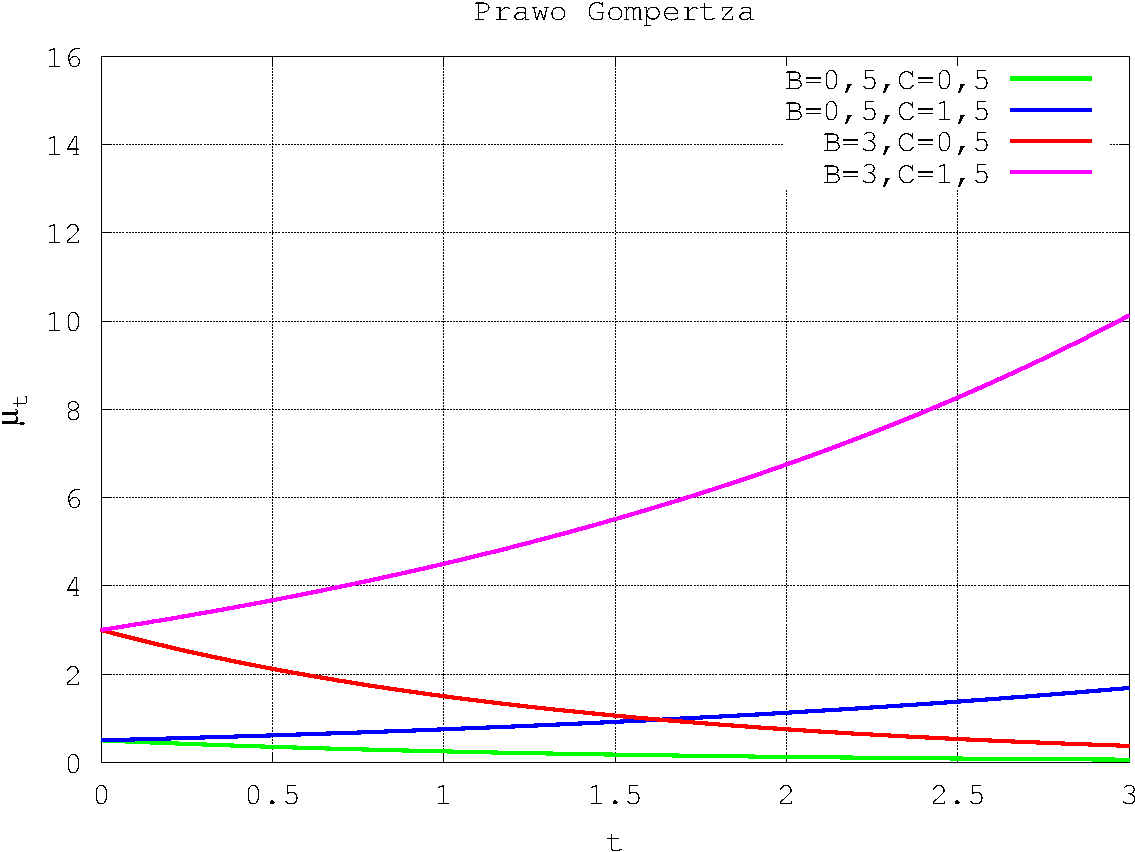
\includegraphics[width=0.9\linewidth]{rys/gom-crop.pdf}
  \caption{Natężenie śmiertelności $\mu_t$ w~modelu Gompertza}
  \label{fig:gompertz}
  \zrodlo{Opracowanie własne}
\end{figure}


\begin{figure}[htpb]
	\centering
		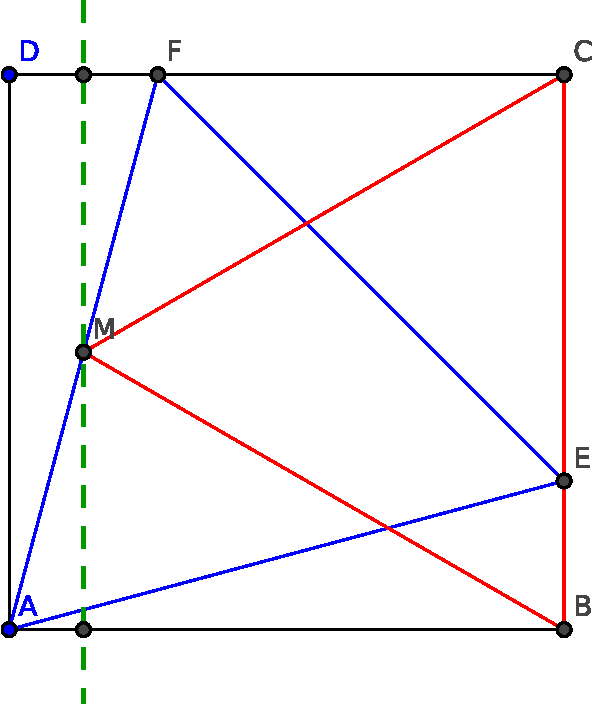
\includegraphics{rys/kwadracik.pdf}
	\caption{Kwadracik, ilustrujący rozwiązanie zadania}
	\label{fig:kwadracik}
	\zrodlo{\cite{Zenner2001}}
\end{figure}

Na rysunku~\ref{fig:kwadracik} możemy zauważyć dwa trójkąty równoboczne. Wielkie mi odkrycie.
Nie ma zatem takiego człowieka, który kocha cierpienie samo w sobie, 
kto by do niego dążył lub chciał go doświadczyć, tylko dlatego, że
jest to cierpienie, a dlatego, że czasami zdarzają się takie 
okoliczności, w których to cierpienie może doprowadzić 
go do jakiejś wielkiej przyjemności. 
Dając przykład banalny: któż z nas kiedyś nie podejmował 
się trudnego wysiłku fizycznego mając na względzie 
uzyskanie z tego korzyści? 
Kto ma jakiekolwiek prawo obwiniać człowieka, 
który wybiera przyjemność nie wiążącą się z~przykrymi 
konsekwencjami, albo tego, kto unika takiego cierpienia, 
które nie prowadzi do przyjemności? 
Jednocześnie potępiamy ze słusznym oburzeniem i czujemy 
niechęć do ludzi, którzy są tak owładnięci urokami nietrwałej 
przyjemności, tak zaślepieni jej pragnieniem, 
że nie dostrzegają, iż następstwem ich 
postępowania będą z pewnością cierpienie i trudności.

Nie ma zatem takiego człowieka, który kocha cierpienie samo w sobie, 
kto by do niego dążył lub chciał go doświadczyć, tylko dlatego, że
jest to cierpienie, a dlatego, że czasami zdarzają się takie 
okoliczności, w których to cierpienie może doprowadzić 
go do jakiejś wielkiej przyjemności. 
Dając przykład banalny: któż z nas kiedyś nie podejmował 
się trudnego wysiłku fizycznego mając na względzie 
uzyskanie z tego korzyści? 
Kto ma jakiekolwiek prawo obwiniać człowieka, 
który wybiera przyjemność nie wiążącą się z~przykrymi 
konsekwencjami, albo tego, kto unika takiego cierpienia, 
które nie prowadzi do przyjemności? 
Jednocześnie potępiamy ze słusznym oburzeniem i czujemy 
niechęć do ludzi, którzy są tak owładnięci urokami nietrwałej 
przyjemności, tak zaślepieni jej pragnieniem, 
że nie dostrzegają, iż następstwem ich 
postępowania będą z pewnością cierpienie i trudności.

Nie ma zatem takiego człowieka, który kocha cierpienie samo w sobie, 
kto by do niego dążył lub chciał go doświadczyć, tylko dlatego, że
jest to cierpienie, a dlatego, że czasami zdarzają się takie 
okoliczności, w których to cierpienie może doprowadzić 
go do jakiejś wielkiej przyjemności. 
Dając przykład banalny: któż z nas kiedyś nie podejmował 
się trudnego wysiłku fizycznego mając na względzie 
uzyskanie z tego korzyści? 
Kto ma jakiekolwiek prawo obwiniać człowieka, 
który wybiera przyjemność nie wiążącą się z~przykrymi 
konsekwencjami, albo tego, kto unika takiego cierpienia, 
które nie prowadzi do przyjemności? 
Jednocześnie potępiamy ze słusznym oburzeniem i czujemy 
niechęć do ludzi, którzy są tak owładnięci urokami nietrwałej 
przyjemności, tak zaślepieni jej pragnieniem, 
że nie dostrzegają, iż następstwem ich 
postępowania będą z pewnością cierpienie i trudności.

Nie ma zatem takiego człowieka, który kocha cierpienie samo w sobie, 
kto by do niego dążył lub chciał go doświadczyć, tylko dlatego, że
jest to cierpienie, a dlatego, że czasami zdarzają się takie 
okoliczności, w których to cierpienie może doprowadzić 
go do jakiejś wielkiej przyjemności. 
Dając przykład banalny: któż z nas kiedyś nie podejmował 
się trudnego wysiłku fizycznego mając na względzie 
uzyskanie z tego korzyści? 
Kto ma jakiekolwiek prawo obwiniać człowieka, 
który wybiera przyjemność nie wiążącą się z~przykrymi 
konsekwencjami, albo tego, kto unika takiego cierpienia, 
które nie prowadzi do przyjemności? 
Jednocześnie potępiamy ze słusznym oburzeniem i czujemy 
niechęć do ludzi, którzy są tak owładnięci urokami nietrwałej 
przyjemności, tak zaślepieni jej pragnieniem, 
że nie dostrzegają, iż następstwem ich 
postępowania będą z pewnością cierpienie i trudności.

Nie ma zatem takiego człowieka, który kocha cierpienie samo w sobie, 
kto by do niego dążył lub chciał go doświadczyć, tylko dlatego, że
jest to cierpienie, a dlatego, że czasami zdarzają się takie 
okoliczności, w których to cierpienie może doprowadzić 
go do jakiejś wielkiej przyjemności. 
Dając przykład banalny: któż z nas kiedyś nie podejmował 
się trudnego wysiłku fizycznego mając na względzie 
uzyskanie z tego korzyści? 
Kto ma jakiekolwiek prawo obwiniać człowieka, 
który wybiera przyjemność nie wiążącą się z~przykrymi 
konsekwencjami, albo tego, kto unika takiego cierpienia, 
które nie prowadzi do przyjemności? 
Jednocześnie potępiamy ze słusznym oburzeniem i czujemy 
niechęć do ludzi, którzy są tak owładnięci urokami nietrwałej 
przyjemności, tak zaślepieni jej pragnieniem, 
że nie dostrzegają, iż następstwem ich 
postępowania będą z pewnością cierpienie i trudności.


Nie ma zatem takiego człowieka, który kocha cierpienie samo w sobie, 
kto by do niego dążył lub chciał go doświadczyć, tylko dlatego, że
jest to cierpienie, a dlatego, że czasami zdarzają się takie 
okoliczności, w których to cierpienie może doprowadzić 
go do jakiejś wielkiej przyjemności. 
Dając przykład banalny: któż z nas kiedyś nie podejmował 
się trudnego wysiłku fizycznego mając na względzie 
uzyskanie z tego korzyści? 
Kto ma jakiekolwiek prawo obwiniać człowieka, 
który wybiera przyjemność nie wiążącą się z~przykrymi 
konsekwencjami, albo tego, kto unika takiego cierpienia, 
które nie prowadzi do przyjemności? 
Jednocześnie potępiamy ze słusznym oburzeniem i czujemy 
niechęć do ludzi, którzy są tak owładnięci urokami nietrwałej 
przyjemności, tak zaślepieni jej pragnieniem, 
że nie dostrzegają, iż następstwem ich 
postępowania będą z pewnością cierpienie i trudności.

Nie ma zatem takiego człowieka, który kocha cierpienie samo w sobie, 
kto by do niego dążył lub chciał go doświadczyć, tylko dlatego, że
jest to cierpienie, a dlatego, że czasami zdarzają się takie 
okoliczności, w których to cierpienie może doprowadzić 
go do jakiejś wielkiej przyjemności. 
Dając przykład banalny: któż z nas kiedyś nie podejmował 
się trudnego wysiłku fizycznego mając na względzie 
uzyskanie z tego korzyści? 
Kto ma jakiekolwiek prawo obwiniać człowieka, 
który wybiera przyjemność nie wiążącą się z~przykrymi 
konsekwencjami, albo tego, kto unika takiego cierpienia, 
które nie prowadzi do przyjemności? 
Jednocześnie potępiamy ze słusznym oburzeniem i czujemy 
niechęć do ludzi, którzy są tak owładnięci urokami nietrwałej 
przyjemności, tak zaślepieni jej pragnieniem, 
że nie dostrzegają, iż następstwem ich 
postępowania będą z pewnością cierpienie i trudności.

Nie ma zatem takiego człowieka, który kocha cierpienie samo w sobie, 
kto by do niego dążył lub chciał go doświadczyć, tylko dlatego, że
jest to cierpienie, a dlatego, że czasami zdarzają się takie 
okoliczności, w których to cierpienie może doprowadzić 
go do jakiejś wielkiej przyjemności. 
Dając przykład banalny: któż z nas kiedyś nie podejmował 
się trudnego wysiłku fizycznego mając na względzie 
uzyskanie z tego korzyści? 
Kto ma jakiekolwiek prawo obwiniać człowieka, 
który wybiera przyjemność nie wiążącą się z~przykrymi 
konsekwencjami, albo tego, kto unika takiego cierpienia, 
które nie prowadzi do przyjemności? 
Jednocześnie potępiamy ze słusznym oburzeniem i czujemy 
niechęć do ludzi, którzy są tak owładnięci urokami nietrwałej 
przyjemności, tak zaślepieni jej pragnieniem, 
że nie dostrzegają, iż następstwem ich 
postępowania będą z pewnością cierpienie i trudności.



\chapter*{Podsumowanie i~wnioski}

Nie ma zatem takiego człowieka, który kocha cierpienie samo w sobie, 
kto by do niego dążył lub chciał go doświadczyć, tylko dlatego, że
jest to cierpienie, a dlatego, że czasami zdarzają się takie 
okoliczności, w których to cierpienie może doprowadzić 
go do jakiejś wielkiej przyjemności. 
Dając przykład banalny: któż z nas kiedyś nie podejmował 
się trudnego wysiłku fizycznego mając na względzie 
uzyskanie z tego korzyści? 
Kto ma jakiekolwiek prawo obwiniać człowieka, 
który wybiera przyjemność nie wiążącą się z~przykrymi 
konsekwencjami, albo tego, kto unika takiego cierpienia, 
które nie prowadzi do przyjemności? 
Jednocześnie potępiamy ze słusznym oburzeniem i czujemy 
niechęć do ludzi, którzy są tak owładnięci urokami nietrwałej 
przyjemności, tak zaślepieni jej pragnieniem, 
że nie dostrzegają, iż następstwem ich 
postępowania będą z pewnością cierpienie i trudności.

Nie ma zatem takiego człowieka, który kocha cierpienie samo w sobie, 
kto by do niego dążył lub chciał go doświadczyć, tylko dlatego, że
jest to cierpienie, a dlatego, że czasami zdarzają się takie 
okoliczności, w których to cierpienie może doprowadzić 
go do jakiejś wielkiej przyjemności. 
Dając przykład banalny: któż z nas kiedyś nie podejmował 
się trudnego wysiłku fizycznego mając na względzie 
uzyskanie z tego korzyści? 
Kto ma jakiekolwiek prawo obwiniać człowieka, 
który wybiera przyjemność nie wiążącą się z~przykrymi 
konsekwencjami, albo tego, kto unika takiego cierpienia, 
które nie prowadzi do przyjemności? 
Jednocześnie potępiamy ze słusznym oburzeniem i czujemy 
niechęć do ludzi, którzy są tak owładnięci urokami nietrwałej 
przyjemności, tak zaślepieni jej pragnieniem, 
że nie dostrzegają, iż następstwem ich 
postępowania będą z pewnością cierpienie i trudności.

Nie ma zatem takiego człowieka, który kocha cierpienie samo w sobie, 
kto by do niego dążył lub chciał go doświadczyć, tylko dlatego, że
jest to cierpienie, a dlatego, że czasami zdarzają się takie 
okoliczności, w których to cierpienie może doprowadzić 
go do jakiejś wielkiej przyjemności. 
Dając przykład banalny: któż z nas kiedyś nie podejmował 
się trudnego wysiłku fizycznego mając na względzie 
uzyskanie z tego korzyści? 
Kto ma jakiekolwiek prawo obwiniać człowieka, 
który wybiera przyjemność nie wiążącą się z~przykrymi 
konsekwencjami, albo tego, kto unika takiego cierpienia, 
które nie prowadzi do przyjemności? 
Jednocześnie potępiamy ze słusznym oburzeniem i czujemy 
niechęć do ludzi, którzy są tak owładnięci urokami nietrwałej 
przyjemności, tak zaślepieni jej pragnieniem, 
że nie dostrzegają, iż następstwem ich 
postępowania będą z pewnością cierpienie i trudności.

Nie ma zatem takiego człowieka, który kocha cierpienie samo w sobie, 
kto by do niego dążył lub chciał go doświadczyć, tylko dlatego, że
jest to cierpienie, a dlatego, że czasami zdarzają się takie 
okoliczności, w których to cierpienie może doprowadzić 
go do jakiejś wielkiej przyjemności. 
Dając przykład banalny: któż z nas kiedyś nie podejmował 
się trudnego wysiłku fizycznego mając na względzie 
uzyskanie z tego korzyści? 
Kto ma jakiekolwiek prawo obwiniać człowieka, 
który wybiera przyjemność nie wiążącą się z~przykrymi 
konsekwencjami, albo tego, kto unika takiego cierpienia, 
które nie prowadzi do przyjemności? 
Jednocześnie potępiamy ze słusznym oburzeniem i czujemy 
niechęć do ludzi, którzy są tak owładnięci urokami nietrwałej 
przyjemności, tak zaślepieni jej pragnieniem, 
że nie dostrzegają, iż następstwem ich 
postępowania będą z pewnością cierpienie i trudności.

\begin{thebibliography}{99}


\bibitem{Beth1984}
T. Beth, F. C. Piper, \emph{The Stop-and-Go Generator} Advances in Cryptology -- EUROCRYPT '84, LNCS vol.~209, pp.~88--92, Springer-Verlag, 1985

\bibitem{Gollmann1989}
W. Chambers, D. Gollmann, \emph{Clock-Controlled Shift Registers: A~Review} IEEE J. Selected Areas Comm., 7(4):~525--533, May 1989
P. R. Geffe, \emph{How to Protect Data with Ciphers That Are Really Hard to Break} Electronics, Jan. 4, pp.~99--10, 1973


\bibitem{Golic1994}
Jovan Dj. Goli\v{c}, Luke O'Connor, \emph{Embedding and Probabilistic Correlation Attacks on Clock-Controlled Shift Registers} Advances in Cryptology -- EUROCRYPT '94, LNCS vol.~950, pp.~230--243, Springer-Verlag, 1995

\bibitem{Zenner2001}
Matthias Krause, Stefan Lucks, Erik Zenner, \emph{Improved
Cryptanalysis of the Self-Shrinking Generator} Information Security
and Privacy -- ACISP 2001, LNCS vol.~2119, pp.~21--35,
Springer-Verlag, 2001.

\bibitem{Meier1994}
W. Meier, O. Staffelbach, \emph{The Self-shrinking Generator} Advances
in Cryptology -- EUROCRYPT '94, LNCS vol.~950, pp.~205--214,
Springer\dywiz Verlag, 1995.

\bibitem{Mihaljevic1996}
Miodrag Mihaljevic, \emph{A Faster Cryptanalysis of the Self-shrinking
Generator} Information Security and Privacy -- ACISP '96, LNCS
vol.~1172, pp.~182--188, Springer\dywiz Verlag, 1996.

\bibitem{Otto04}
W.~Otto, \emph{Ubezpieczenia majątkowe. Część I Teoria ryzyka},
Wydawnictwo Naukowo-Techniczne, Warszawa 2004.

\bibitem{Zeng1991}
T. R. N. Rao, Chung-Huang Yang, Kencheng Zeng, \emph{An Improved
Linear Syndrome Algorithm in Cryptanalysis With Applications} Advances
in Cryptology -- CRYPTO '90, LNCS vol.~537, pp.~34--47,
Springer\dywiz Verlag, 1991.


\bibitem{Zenner2002}
Erik Zenner, \emph{On the Efficiency of the Clock Control Guessing
Attack} Information Security and Cryptology -- ICISC 2002, LNCS
vol.~2587, pp.~200--212, Springer\dywiz Verlag, 2003.

\bibitem{Szekli11}
R.~Dutak, W.~Wzekly, \emph{Matematyka ubezpieczeń majątkowych},
Uniwersytet Paragwajski,
\url{http://www.math.uni.up/gracias/seniores}, \emph{stan w~dniu
5.03.2012~r.}

\end{thebibliography}



\listoffigures

\listoftables


\chapter*{Załączniki}
\begin{enumerate}
\item Płyta CD z niniejszą pracą w wersji elektronicznej.
\item Oświadczenie o oryginalności pracy i możliwości jej wykorzystania. 
\end{enumerate}




\chapter*{Streszczenie (Summary)}

\bigskip
\bigskip

\begin{center}
  \textbf{\tytul}
\end{center}


Nie ma zatem takiego człowieka, który kocha cierpienie samo w sobie, 
kto by do niego dążył lub chciał go doświadczyć, tylko dlatego, że
jest to cierpienie, a dlatego, że czasami zdarzają się takie 
okoliczności, w których to cierpienie może doprowadzić 
go do jakiejś wielkiej przyjemności. 
Dając przykład banalny: któż z nas kiedyś nie podejmował 
się trudnego wysiłku fizycznego mając na względzie 
uzyskanie z tego korzyści? 
Kto ma jakiekolwiek prawo obwiniać człowieka, 
który wybiera przyjemność nie wiążącą się z~przykrymi 
konsekwencjami, albo tego, kto unika takiego cierpienia, 
które nie prowadzi do przyjemności? 
Jednocześnie potępiamy ze słusznym oburzeniem i czujemy 
niechęć do ludzi, którzy są tak owładnięci urokami nietrwałej 
przyjemności, tak zaślepieni jej pragnieniem, 
że nie dostrzegają, iż następstwem ich 
postępowania będą z pewnością cierpienie i trudności.

\bigskip

\begin{center}
  \textbf{\textit{\tytulangielski}}
\end{center}


{\it
Nor again is there anyone who loves or pursues or desires to obtain
pain of itself, because it is pain, but because occasionally
circumstances occur in which toil and pain can procure him some great
pleasure. To take a trivial example, which of us ever undertakes
laborious physical exercise, except to obtain some advantage from it?
But who has any right to find fault with a man who chooses to enjoy a
pleasure that has no annoying consequences, or one who avoids a pain
that produces no resultant pleasure?
On the other hand, we denounce with righteous indignation and dislike
men who are so beguiled and demoralized by the charms of pleasure of
the moment, so blinded by desire, that they cannot foresee the pain
and trouble that are bound to ensue.
}

\end{document}

